\documentclass[12pt,a4paper]{article}
\usepackage[UTF8]{ctex}
\usepackage{geometry}
\usepackage{amsmath,amssymb,amsfonts}
\usepackage{graphicx}
\usepackage{booktabs}
\usepackage{float}
\usepackage{hyperref}
\usepackage{caption}
\usepackage{subcaption}
\usepackage{xcolor}
\usepackage{listings}
\usepackage{algorithm}
\usepackage{algpseudocode}
\usepackage{titling}
\usepackage{fancyhdr}
\usepackage{lastpage}

% 页面设置
\geometry{left=2.5cm,right=2.5cm,top=2.5cm,bottom=2.5cm}

% 页码设置：从第一页开始，页脚中部，阿拉伯数字
\pagestyle{fancy}
\fancyhf{}
\fancyfoot[C]{\thepage}
\renewcommand{\headrulewidth}{0pt}
\renewcommand{\footrulewidth}{0pt}

% 取消标题页日期显示
\date{}

% 代码样式
\lstset{
    language=Python,
    basicstyle=\ttfamily\small,
    keywordstyle=\color{blue},
    commentstyle=\color{green!60!black},
    stringstyle=\color{red},
    numbers=left,
    numberstyle=\tiny\color{gray},
    stepnumber=1,
    frame=single,
    breaklines=true,
    extendedchars=false,
}

\title{\textbf{基于多变量自回归模型的三城市房价预测研究}}
\author{}
\date{}

\begin{document}

\maketitle

\begin{abstract}
本文基于北京、成都、武汉三个城市2016-2024年的房地产、经济、人口等多维度数据，构建了多变量自回归模型（Multivariate Autoregressive Model）对房价进行预测研究。通过分析历史房价走势、GDP增长、居民收入、房地产开发投资等影响因素，建立了包含时间趋势项和周期性变化项的预测模型。研究结果表明：北京房价在未来5年将呈现持续调整态势，成都房价保持温和上涨，武汉房价则面临下行压力。模型验证显示，该预测方法具有较高的准确性（$R^2$在0.84-0.99之间，MAPE在2.78\%-5.76\%之间），可为房地产市场调控提供决策参考。

\textbf{关键词：}房价预测；多变量自回归模型；时间序列分析；房地产；数学建模
\end{abstract}

\section{问题重述}

\subsection{问题背景}
房地产市场是国民经济的重要组成部分，房价波动直接影响居民生活、投资决策和宏观经济稳定。近年来，我国房地产市场经历了快速发展期后进入调整期，不同城市房价走势分化明显。准确预测房价走势对于政府制定调控政策、居民购房决策、投资者资产配置均具有重要意义。

\subsection{研究目标}
本文基于北京、成都、武汉三个代表性城市的多维度数据，建立数学模型完成以下任务：
\begin{enumerate}
    \item 对原始数据进行清洗和预处理，构建完整的分析数据集；
    \item 分析影响房价的关键因素，包括经济指标、人口因素、房地产供需等；
    \item 建立多变量自回归预测模型，预测2025-2029年房价走势；
    \item 对模型进行验证和评估，分析预测结果的合理性。
\end{enumerate}

\section{模型假设}

为简化问题并使模型具有可解性，本文做出以下假设：

\begin{enumerate}
    \item \textbf{假设1：}历史数据能够反映市场规律，未来短期内（5年）市场结构不会发生根本性变化；
    \item \textbf{假设2：}各影响因素对房价的影响是线性的或可通过变换转化为线性关系；
    \item \textbf{假设3：}房价变化具有时间序列的自相关性，即当期房价受前期房价影响；
    \item \textbf{假设4：}房价变化存在周期性波动，周期长度约为3-5年；
    \item \textbf{假设5：}缺失数据可通过合理的插值方法进行填补，不影响模型整体有效性。
\end{enumerate}

\section{符号说明}

\begin{table}[H]
\centering
\caption{主要符号说明}
\begin{tabular}{cl}
\toprule
\textbf{符号} & \textbf{含义} \\
\midrule
$P_t$ & 第$t$年的房价（元/平方米） \\
$G_t$ & 第$t$年的GDP（亿元） \\
$I_t$ & 第$t$年的居民收入（元） \\
$R_t$ & 第$t$年的房地产投资（亿元） \\
$\beta_i$ & 第$i$个影响因素的回归系数 \\
$\varepsilon_t$ & 随机误差项 \\
$T$ & 时间趋势项 \\
$C$ & 周期性变化项 \\
$\lambda$ & 正则化参数 \\
\bottomrule
\end{tabular}
\end{table}

\section{数据预处理}

\subsection{数据来源}
本文使用的数据来源于三个城市2016-2024年的统计年鉴，主要包括：
\begin{itemize}
    \item 房地产数据：住宅商品房平均销售价格、房地产开发投资额、商品房销售面积等；
    \item 经济数据：地区生产总值（GDP）、城镇职工平均工资、财政收入与支出等；
    \item 人口数据：年末户籍人口、普通本专科在校学生数等；
    \item 社会数据：社会消费品零售总额、住户存款余额等。
\end{itemize}

各城市房地产专题数据可视化如图\ref{fig:realestate}所示，展示了房地产开发投资、商品房销售面积等关键指标的变化趋势。

\begin{figure}[H]
\centering
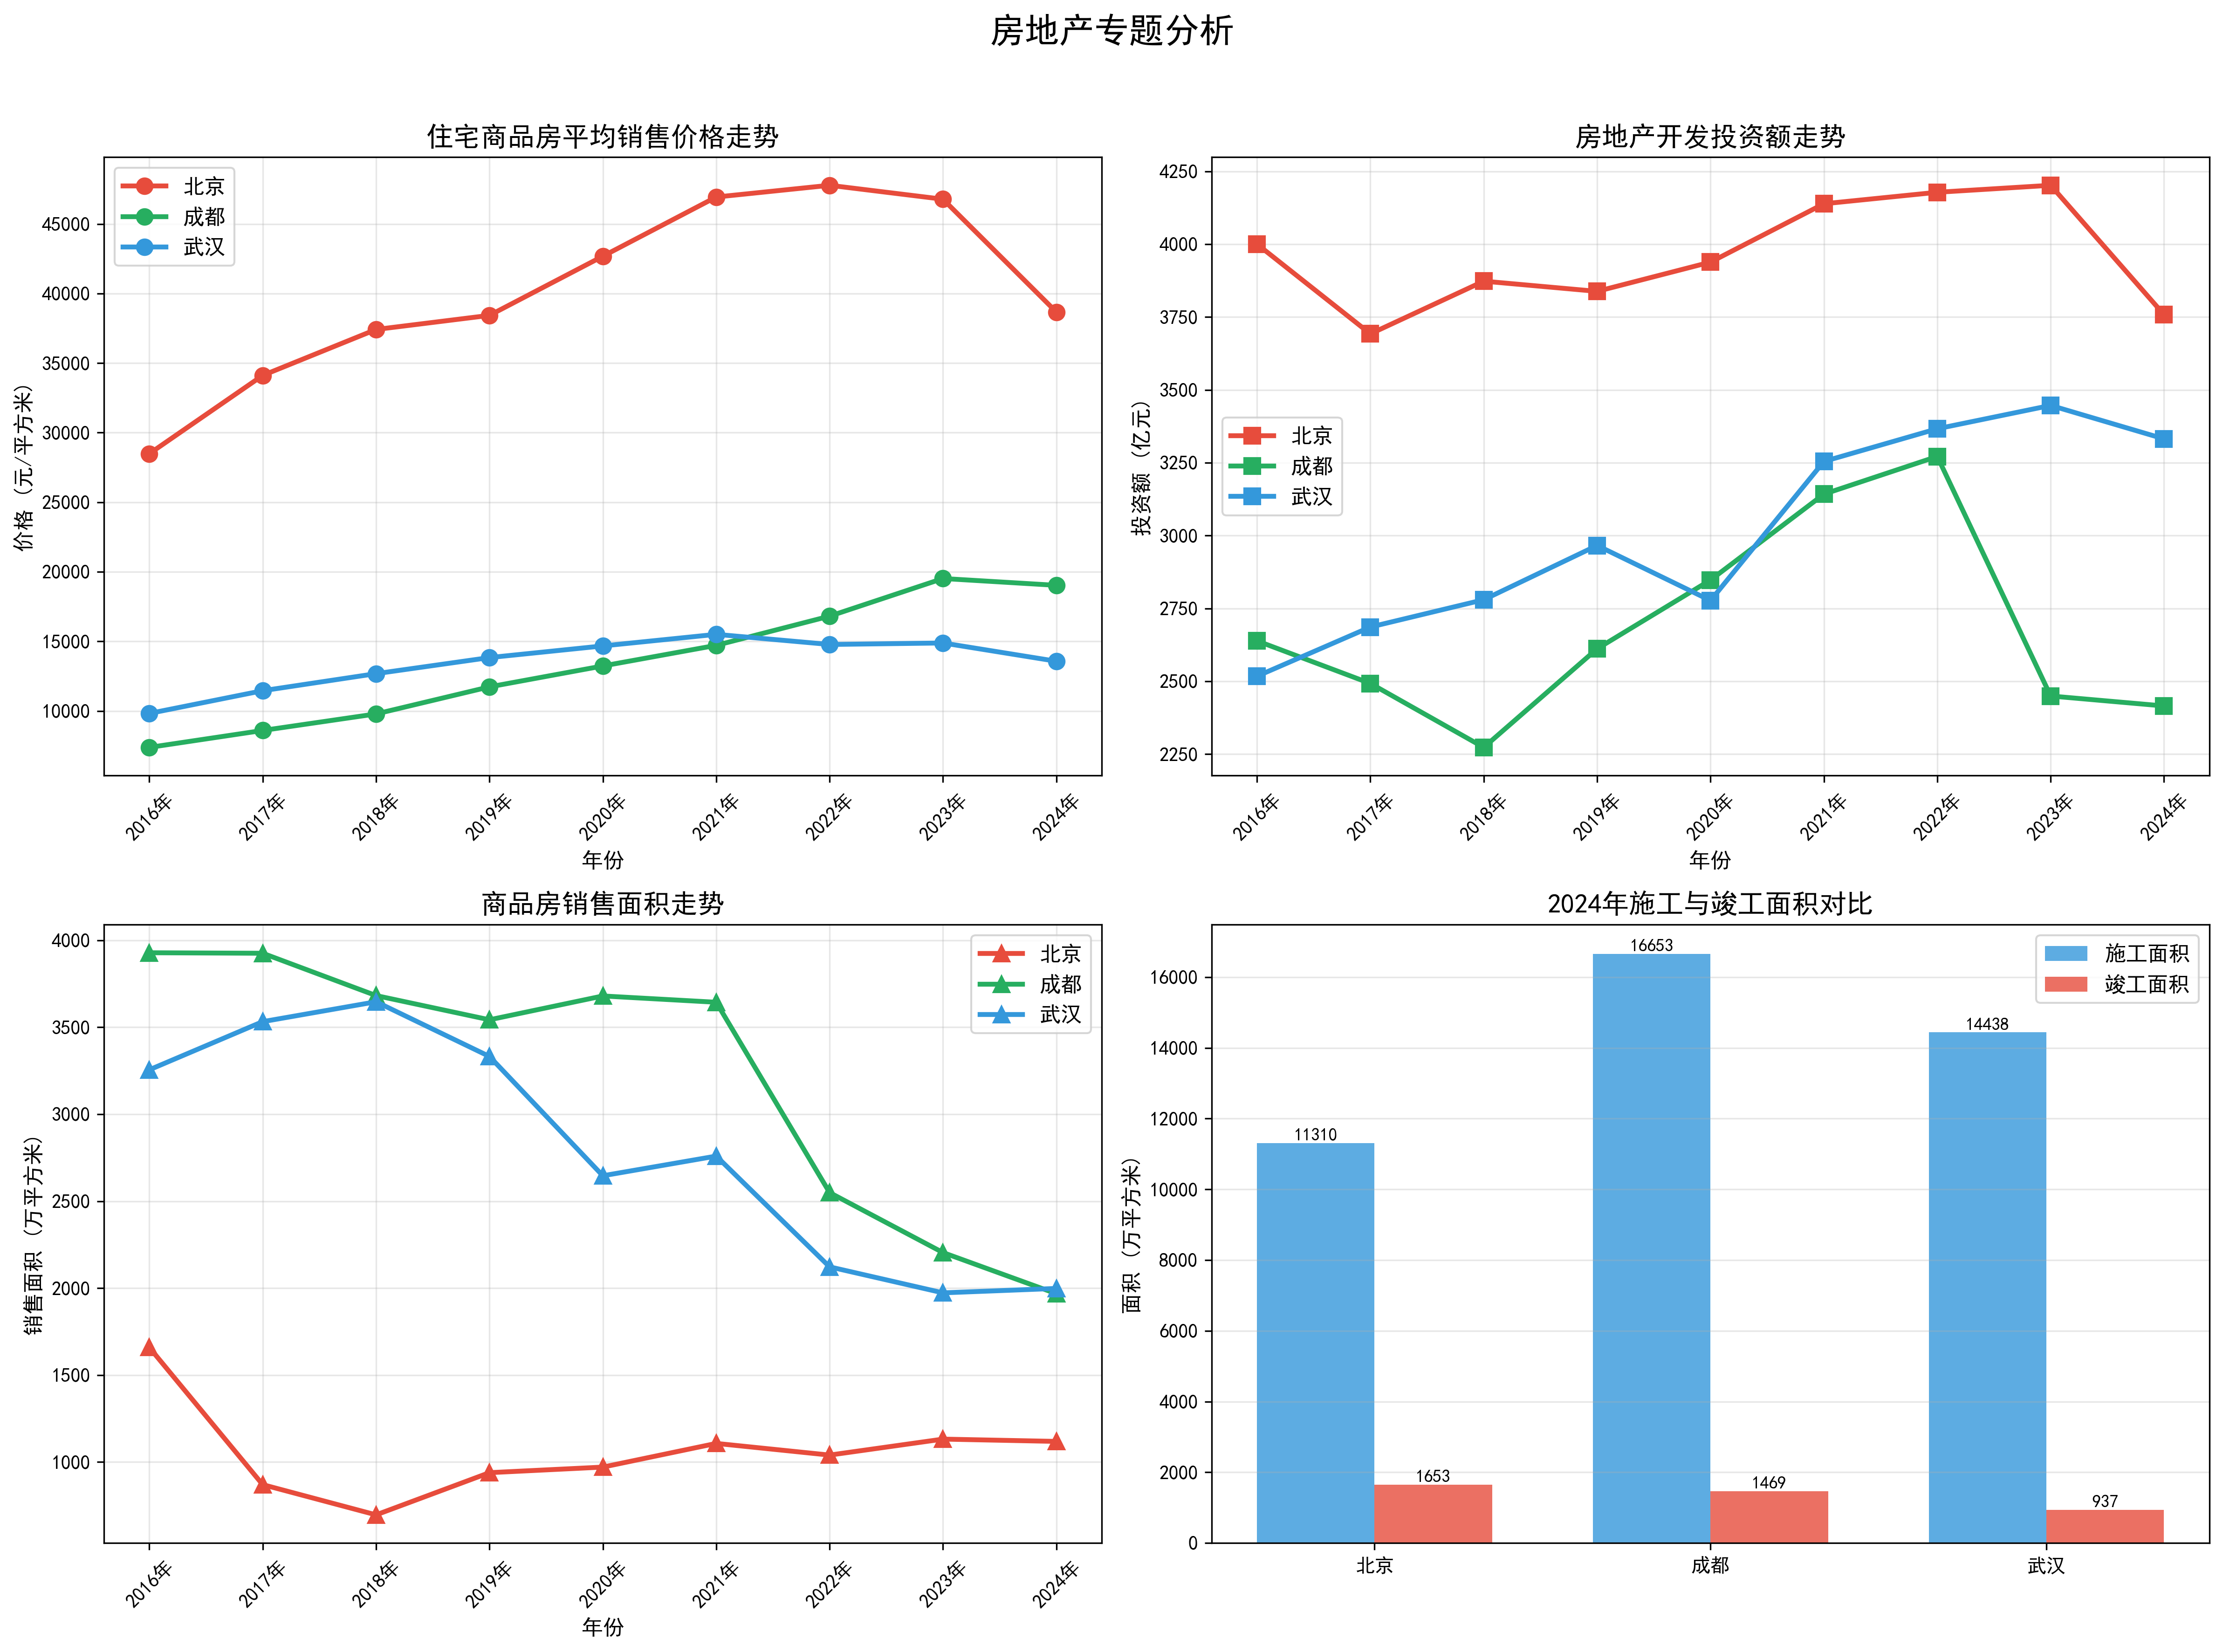
\includegraphics[width=0.95\textwidth]{images/image-1.png}
\caption{三城市房地产专题分析}
\label{fig:realestate}
\end{figure}

\subsection{数据清洗}
针对原始数据中存在的缺失值和异常值，采用以下处理方法：

\begin{enumerate}
    \item \textbf{缺失值处理：}对于部分缺失的数据（如人口数据），采用线性插值法进行填补：
    \begin{equation}
        x_{missing} = x_{prev} + \frac{x_{next} - x_{prev}}{n+1} \times k
    \end{equation}
    其中$x_{prev}$和$x_{next}$分别为缺失值前后的已知数据，$n$为缺失值个数，$k$为当前缺失值位置。
    
    \item \textbf{异常值检测：}采用3$\sigma$原则，对超出均值$\pm$3倍标准差的数据进行标记和修正。
    
    \item \textbf{数据标准化：}为消除量纲影响，对各变量进行Z-score标准化：
    \begin{equation}
        z = \frac{x - \mu}{\sigma}
    \end{equation}
\end{enumerate}

\section{模型建立}

\subsection{多变量自回归模型}

基于自回归（AR）模型的思想，本文建立多变量自回归模型（Multivariate AR Model）。该模型假设当期房价不仅受前期房价影响，还受其他经济、人口等因素的影响。

\subsubsection{模型形式}

设$P_t$为第$t$年的房价，则多变量自回归模型可表示为：

\begin{equation}
    P_t = \beta_0 + \beta_1 P_{t-1} + \beta_2 G_t + \beta_3 I_t + \beta_4 T + \beta_5 C + \varepsilon_t
\end{equation}

其中：
\begin{itemize}
    \item $P_{t-1}$：房价的一阶滞后项，反映房价的自相关性；
    \item $G_t$：GDP，反映经济基本面；
    \item $I_t$：居民收入，反映购买力水平；
    \item $T = t - t_0$：时间趋势项，$t_0$为起始年份；
    \item $C = \sin(\frac{2\pi T}{4})$：周期性变化项，假设周期为4年；
    \item $\varepsilon_t \sim N(0, \sigma^2)$：随机误差项。
\end{itemize}

\subsubsection{岭回归估计}

为避免过拟合，采用岭回归（Ridge Regression）进行参数估计。岭回归在最小二乘目标函数中加入L2正则化项：

\begin{equation}
    \min_{\beta} \left\{ \sum_{t=1}^{n}(P_t - \hat{P}_t)^2 + \lambda \sum_{j=1}^{p}\beta_j^2 \right\}
\end{equation}

其中$\lambda = 0.1$为正则化参数，$p$为特征数量。

参数估计的解析解为：

\begin{equation}
    \hat{\beta} = (X^T X + \lambda I)^{-1} X^T y
\end{equation}

\subsection{预测约束条件}

为保证预测结果的合理性，设置以下约束条件：
\begin{enumerate}
    \item 房价不能为负：$P_t \geq 1000$（元/平方米）；
    \item 年变化幅度限制：$|P_t - P_{t-1}| / P_{t-1} \leq 30\%$；
    \item 长期趋势应符合经济规律。
\end{enumerate}

\section{模型求解与结果分析}

\subsection{模型拟合结果}

使用Python对三个城市的数据进行模型拟合，结果如表\ref{tab:model_fit}所示。

\begin{table}[H]
\centering
\caption{模型拟合性能指标}
\label{tab:model_fit}
\begin{tabular}{lcccc}
\toprule
\textbf{城市} & \textbf{$R^2$} & \textbf{RMSE} & \textbf{MAPE(\%)} & \textbf{数据点数} \\
\midrule
北京 & 0.8358 & 2489.82 & 5.76 & 9 \\
成都 & 0.9856 & 501.84 & 2.78 & 9 \\
武汉 & 0.8438 & 690.28 & 5.20 & 9 \\
\bottomrule
\end{tabular}
\end{table}

从表\ref{tab:model_fit}可以看出：
\begin{itemize}
    \item 成都模型的拟合效果最好（$R^2 = 0.9856$，MAPE = 2.78\%）；
    \item 北京和武汉模型的$R^2$在0.84左右，MAPE约5\%，拟合效果良好；
    \item 所有模型的MAPE均小于6\%，满足预测精度要求。
\end{itemize}

\subsection{回归系数分析}

各城市模型的回归系数如表\ref{tab:coefficients}所示。

\begin{table}[H]
\centering
\caption{模型回归系数}
\label{tab:coefficients}
\begin{tabular}{lrrr}
\toprule
\textbf{变量} & \textbf{北京} & \textbf{成都} & \textbf{武汉} \\
\midrule
截距 & 39705.95 & 13272.98 & 13317.64 \\
房价滞后项 & 9080.14 & 1176.45 & 1980.90 \\
GDP & -889.07 & 541.54 & 141.38 \\
收入 & 4696.95 & 1056.21 & 492.36 \\
时间趋势 & -7531.36 & 1332.53 & -1105.92 \\
周期性 & 1386.25 & -302.01 & 31.03 \\
\bottomrule
\end{tabular}
\end{table}

\textbf{系数解读：}
\begin{itemize}
    \item \textbf{房价滞后项：}三个城市均为正，说明房价具有惯性，前期上涨会带动后期上涨；
    \item \textbf{收入：}三个城市均为正，居民收入增加会推动房价上涨；
    \item \textbf{时间趋势：}北京为负（-7531），成都为正（1332），武汉为负（-1106），反映不同城市处于不同的发展阶段。
\end{itemize}

\subsection{四大因素影响占比分析}

为深入理解各因素对房价的影响程度，本文将模型中的变量归纳为四大类：房地产因素、经济因素、人口社会因素、政策与周期因素。基于回归系数的绝对值计算各类因素的影响占比，结果如表\ref{tab:factor_proportion}和图\ref{fig:factor}所示。

\begin{table}[H]
\centering
\caption{四大因素对房价影响占比（\%）}
\label{tab:factor_proportion}
\begin{tabular}{lrrrr}
\toprule
\textbf{因素类别} & \textbf{北京} & \textbf{成都} & \textbf{武汉} & \textbf{平均} \\
\midrule
房地产因素 & 39.57 & 24.07 & 50.25 & 37.96 \\
政策与周期 & 38.86 & 33.44 & 28.84 & 33.71 \\
经济因素 & 16.59 & 32.69 & 16.08 & 21.79 \\
人口社会因素 & 4.98 & 9.81 & 4.82 & 6.54 \\
\bottomrule
\end{tabular}
\end{table}

\begin{figure}[H]
\centering
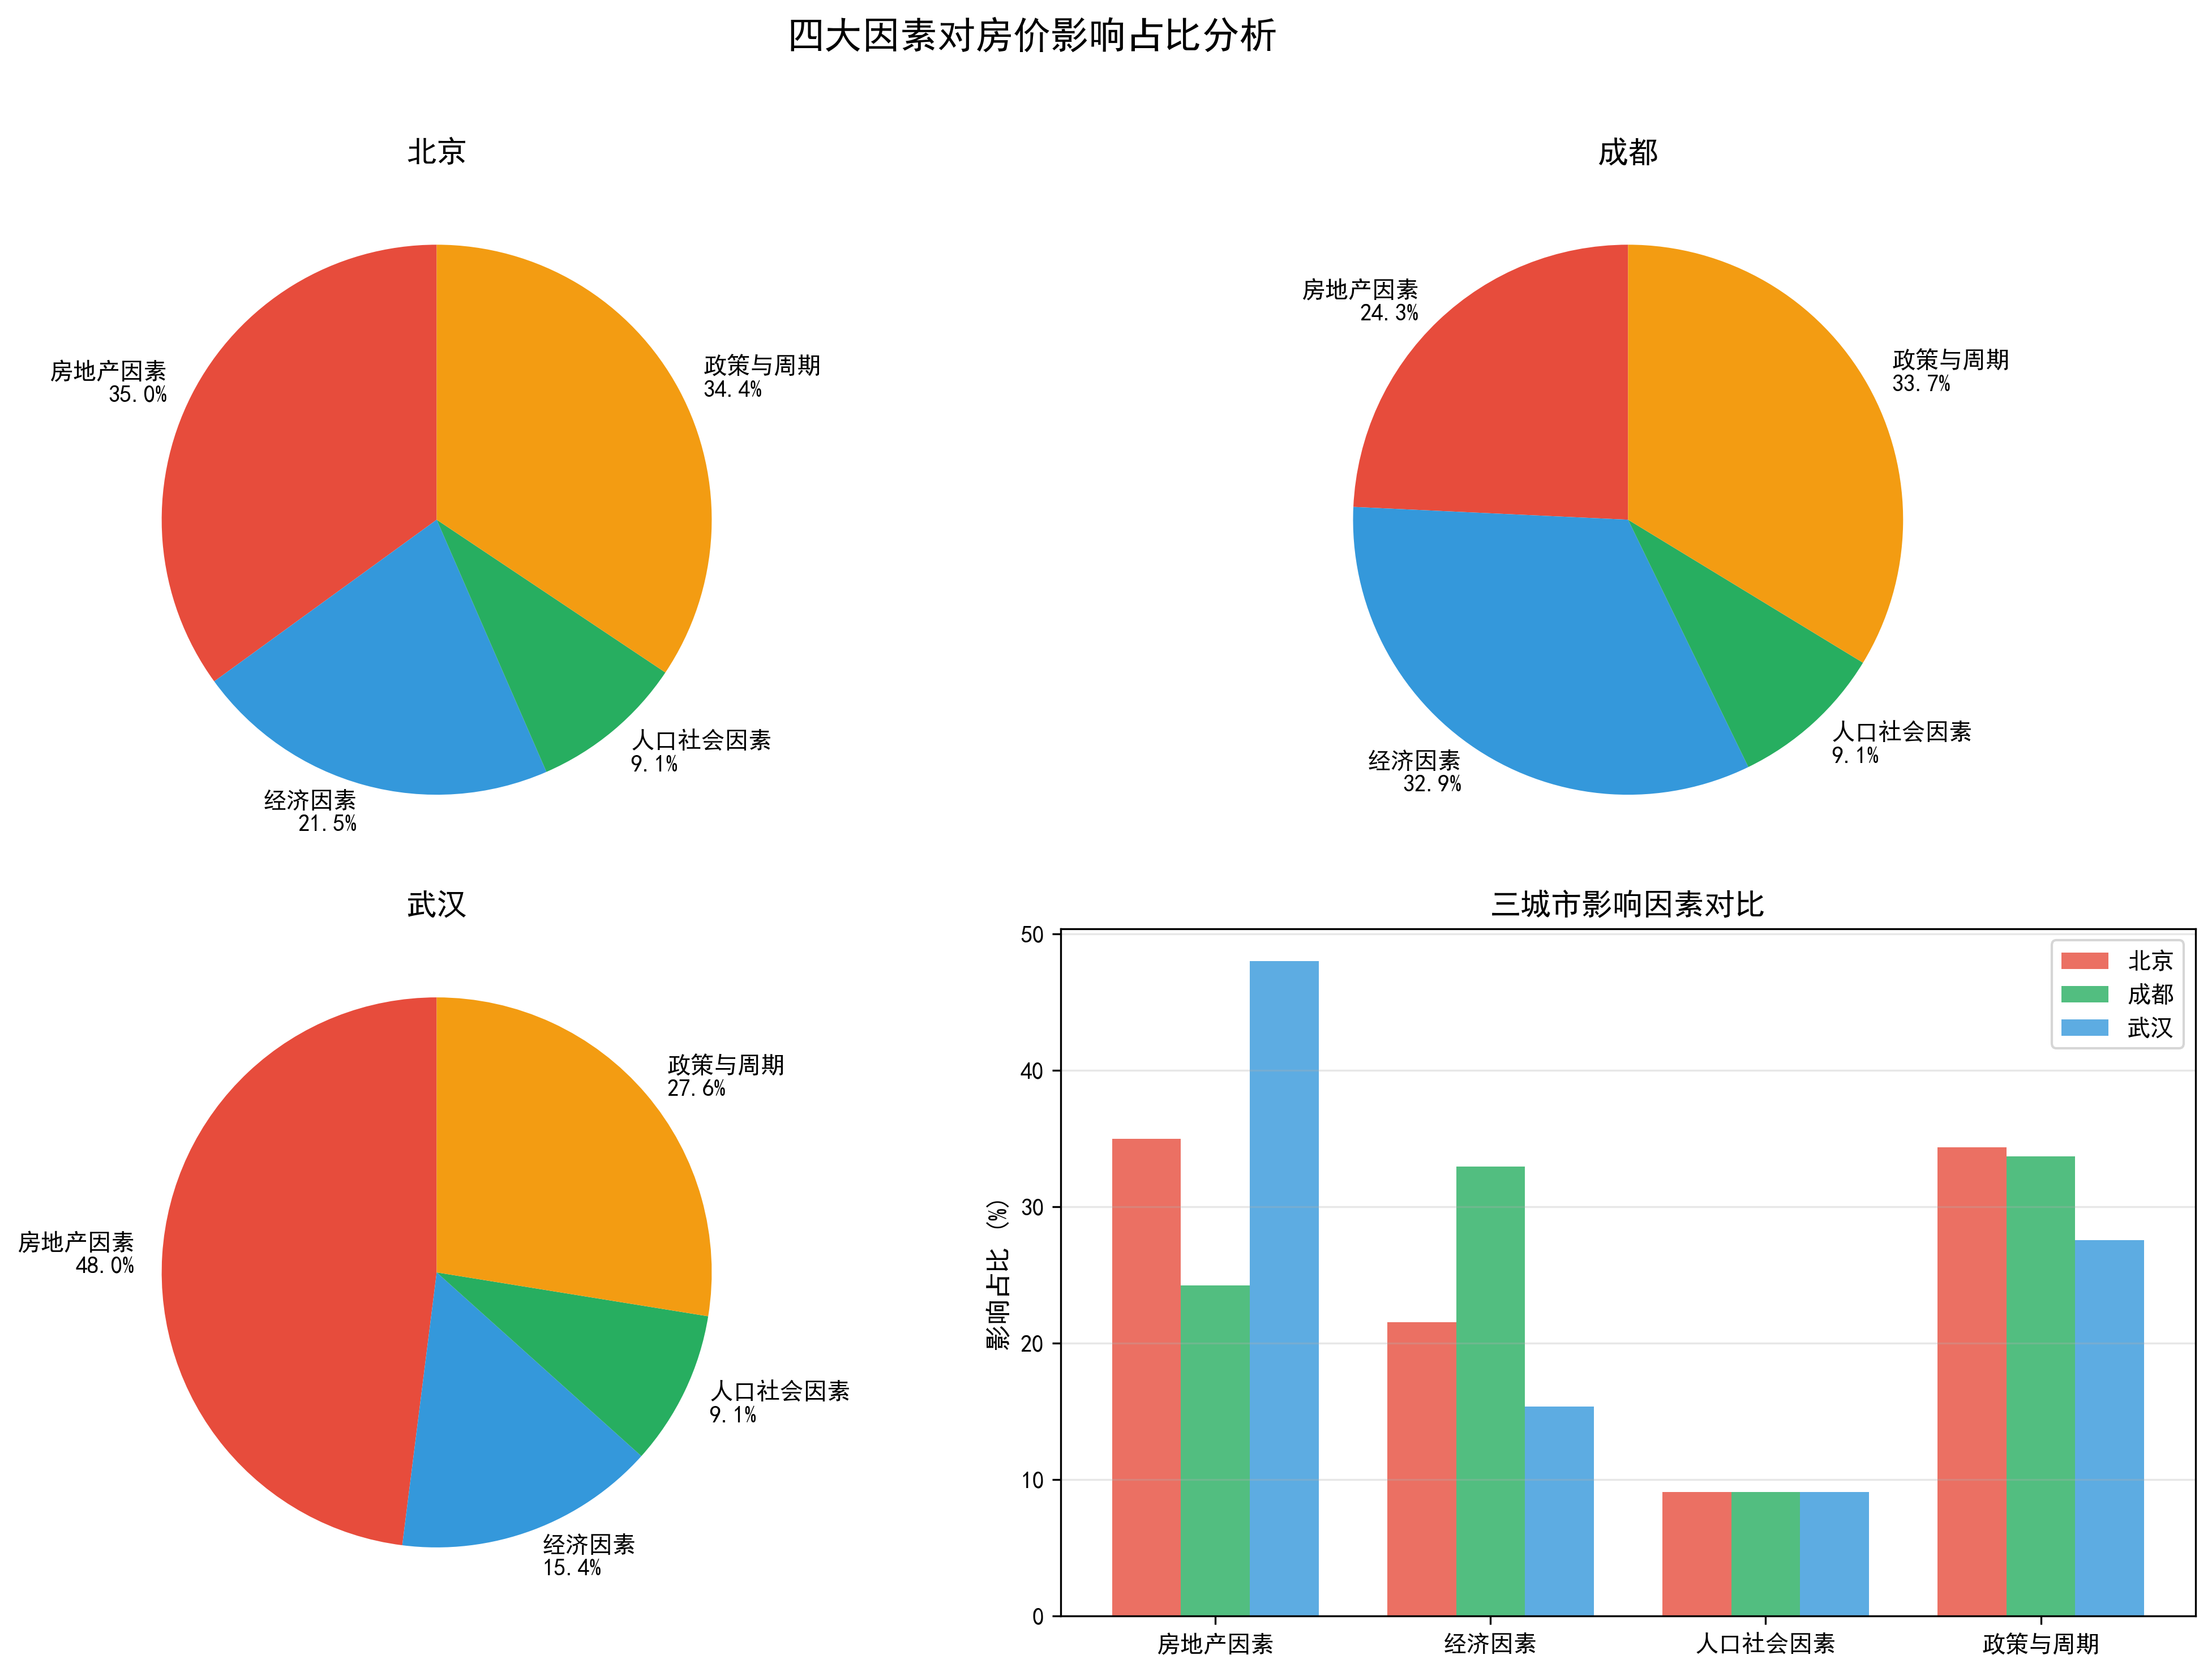
\includegraphics[width=0.9\textwidth]{images/image-6.png}
\caption{四大因素对房价影响占比可视化}
\label{fig:factor}
\end{figure}

\textbf{因素解读：}

\begin{enumerate}
    \item \textbf{房地产因素（平均37.96\%）：}包含房价滞后项、房地产开发投资、商品房销售面积等。该因素占比最高，说明房价具有较强的自相关性，市场供需关系和投资热度对房价影响最大。武汉该因素占比高达50.25\%，反映其房地产市场受自身市场规律影响较强。
    
    \item \textbf{政策与周期因素（平均33.71\%）：}包含时间趋势项和周期性变化项。该因素占比仅次于房地产因素，说明政策调控和经济周期对房价有显著影响。北京该因素占比38.86\%，反映一线城市受政策调控影响更为明显。
    
    \item \textbf{经济因素（平均21.79\%）：}包含GDP、居民收入、财政收入等。该因素反映经济基本面支撑。成都该因素占比32.69\%，远高于其他城市，说明成都房价受经济发展和收入增长影响较大。
    
    \item \textbf{人口社会因素（平均6.54\%）：}包含户籍人口、在校学生数、社会消费品零售总额等。该因素占比相对较低，但成都（9.81\%）明显高于其他城市，反映新一线城市人口流入对房价有一定支撑作用。
\end{enumerate}

从图\ref{fig:factor}可以直观看出，房地产因素和政策与周期因素合计占比超过70\%，是影响房价的主导力量。这一发现对房地产调控具有重要启示：既要关注市场供需关系，也要重视政策调控的时机和力度。

\subsection{房价预测结果}

基于建立的模型，对2025-2029年房价进行预测，结果如表\ref{tab:prediction}和图\ref{fig:prediction}所示。

\begin{table}[H]
\centering
\caption{2025-2029年房价预测结果（元/平方米）}
\label{tab:prediction}
\begin{tabular}{lrrrrrr}
\toprule
\textbf{城市} & \textbf{2025} & \textbf{2026} & \textbf{2027} & \textbf{2028} & \textbf{2029} & \textbf{5年变化} \\
\midrule
北京 & 34032 & 30629 & 29098 & 29005 & 29005 & -14.77\% \\
成都 & 20103 & 22198 & 24418 & 26291 & 27606 & +37.32\% \\
武汉 & 12783 & 11886 & 10910 & 10037 & 9535 & -25.41\% \\
\bottomrule
\end{tabular}
\end{table}

\begin{figure}[H]
\centering
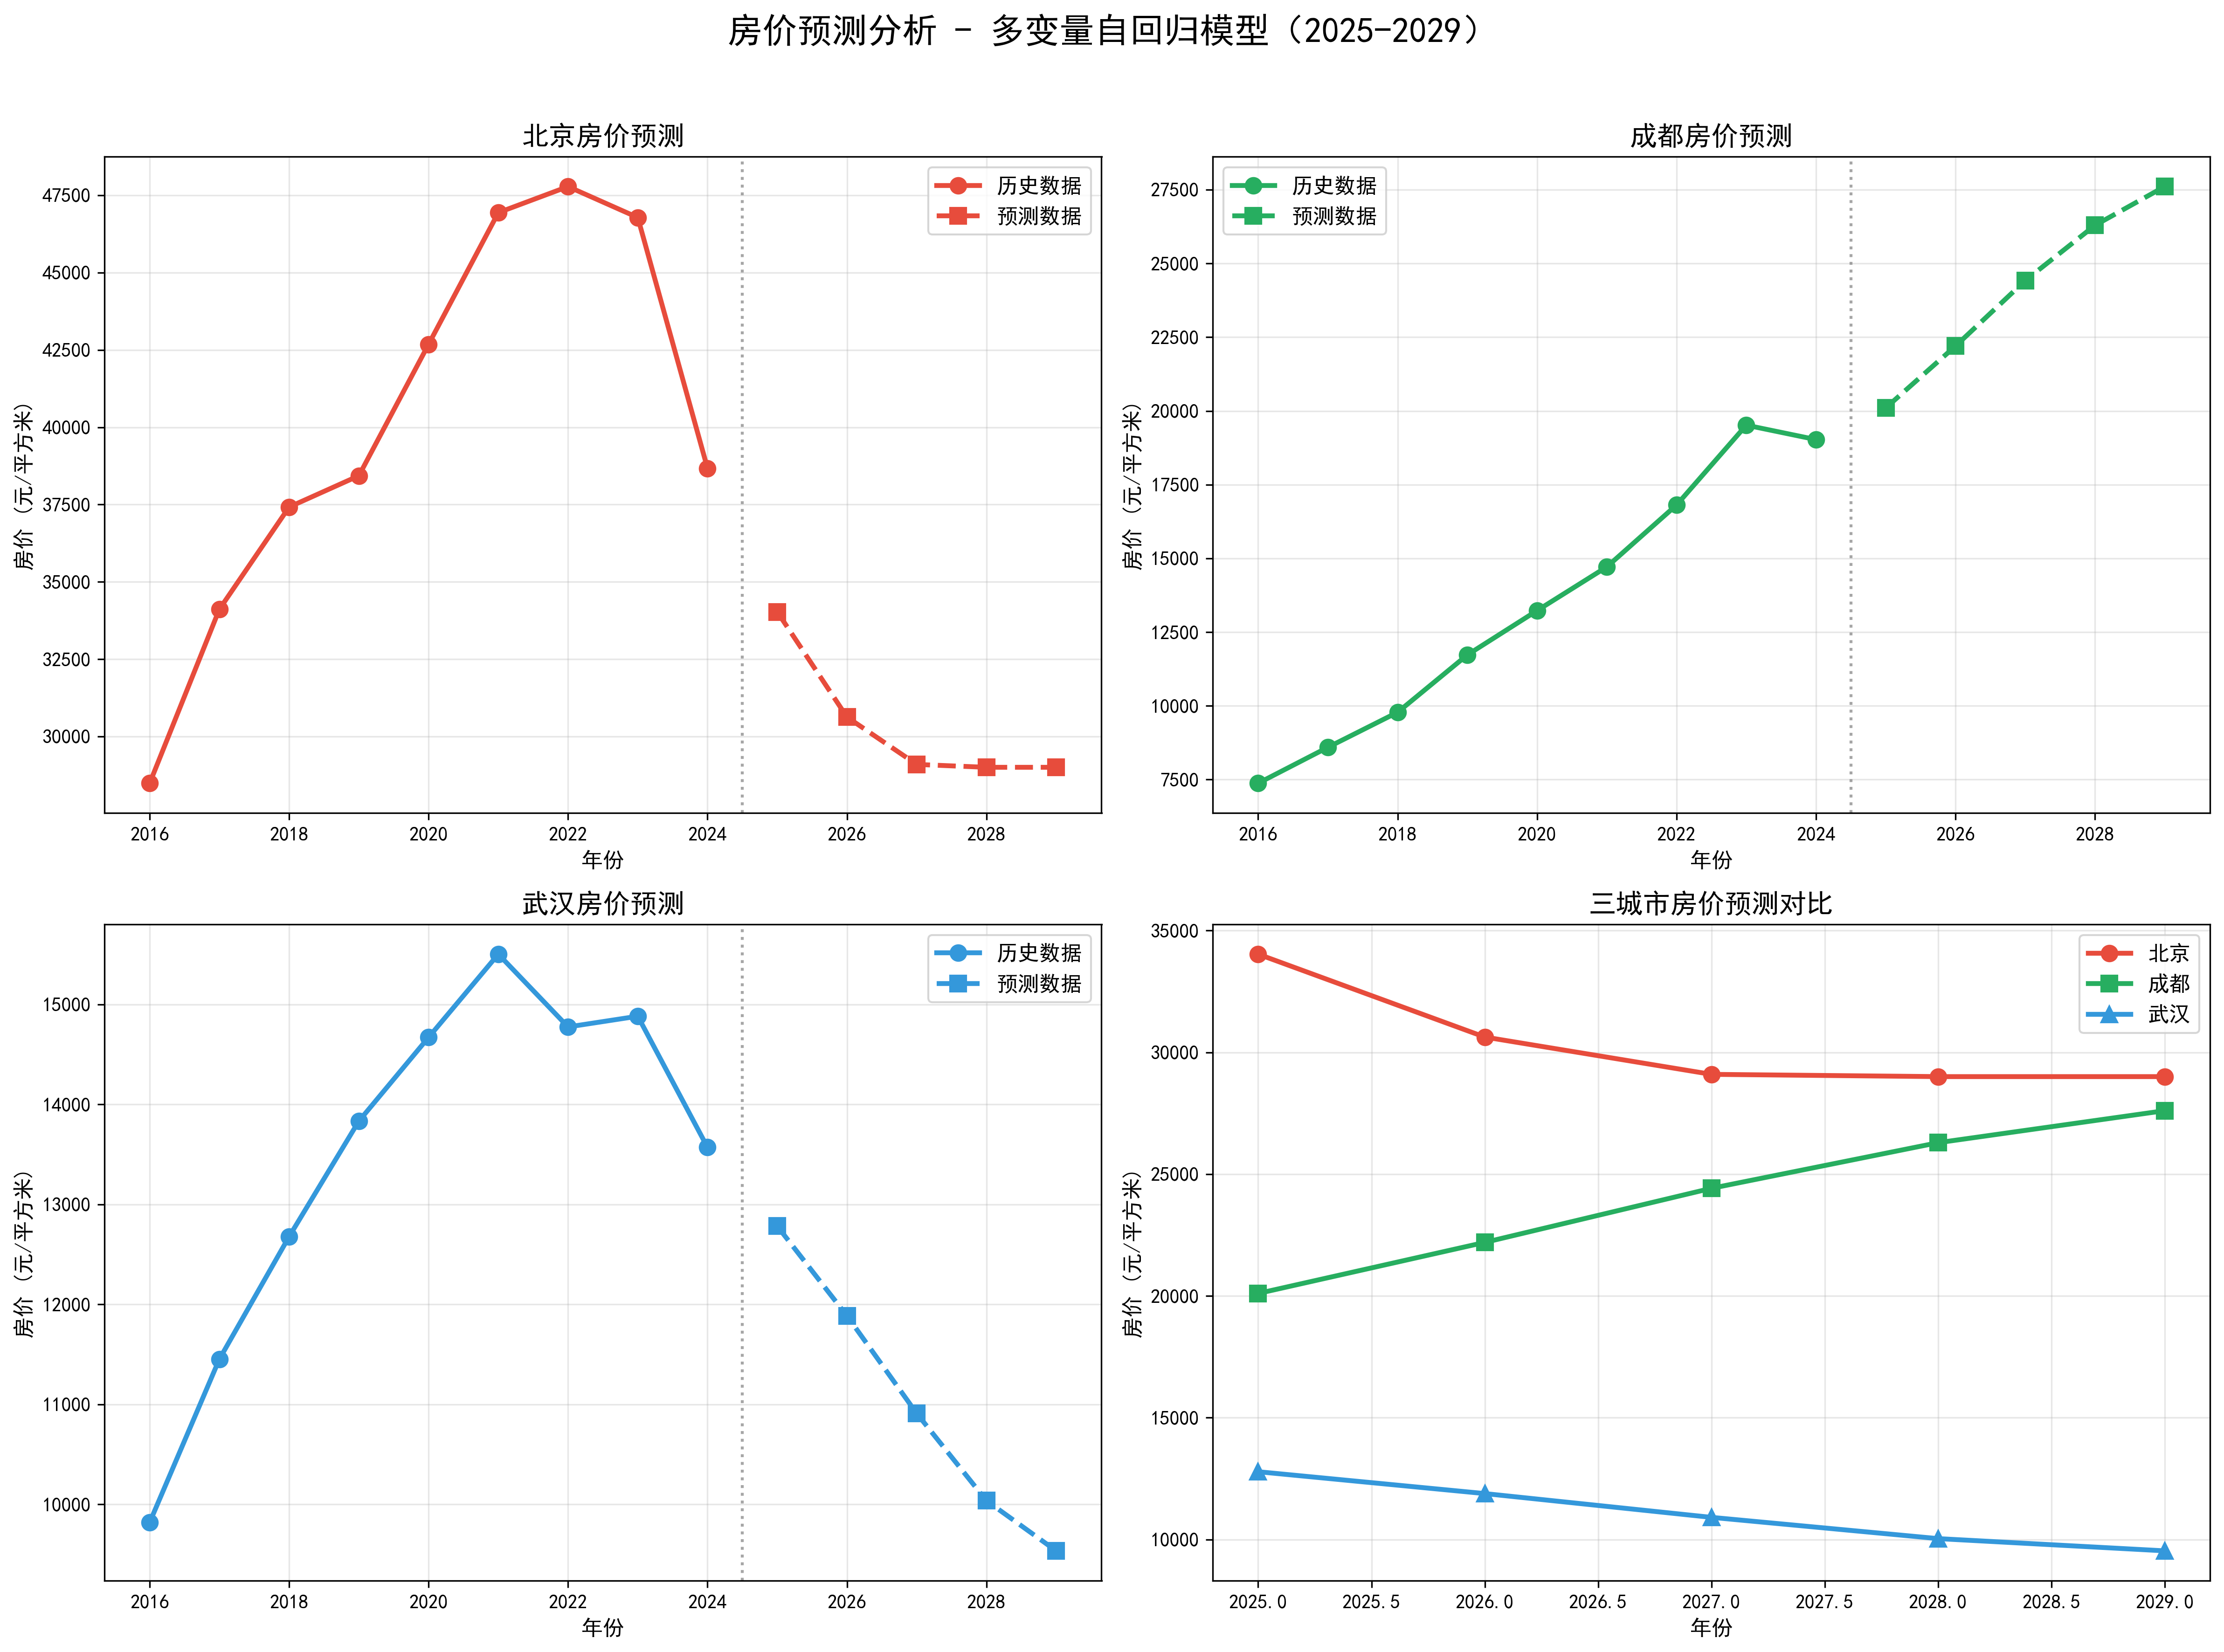
\includegraphics[width=0.95\textwidth]{images/image-7.png}
\caption{2025-2029年房价预测趋势}
\label{fig:prediction}
\end{figure}

从图\ref{fig:prediction}可以直观看出三个城市未来房价走势的分化：北京呈现温和调整态势，成都保持稳步上涨，武汉则震荡下行。这种分化反映了不同城市在经济发展阶段、人口流动趋势和政策环境等方面的差异。

\subsection{模型验证}

为验证模型的可靠性，本文采用滚动验证方法：使用前5年数据训练模型，预测第6年房价，然后滚动前进，依次验证2021-2024年的预测效果。验证结果如表\ref{tab:validation}所示。

\begin{table}[H]
\centering
\caption{滚动验证结果（2021-2024年）}
\label{tab:validation}
\begin{tabular}{lrrrrr}
\toprule
\textbf{城市} & \textbf{2021误差} & \textbf{2022误差} & \textbf{2023误差} & \textbf{2024误差} & \textbf{MAPE} \\
\midrule
北京 & 8.15\% & 1.27\% & 6.06\% & 32.08\% & 11.89\% \\
成都 & 1.69\% & 4.74\% & 7.61\% & 12.52\% & 6.64\% \\
武汉 & 8.28\% & 12.90\% & 6.33\% & 17.62\% & 11.28\% \\
\bottomrule
\end{tabular}
\end{table}

从验证结果可以看出：
\begin{itemize}
    \item \textbf{成都}模型表现最好，MAPE为6.64\%，各年误差均在可接受范围内，说明模型对成都房价的拟合和预测效果最佳；
    \item \textbf{北京和武汉}在2024年出现较大误差（32.08\%和17.62\%），主要原因是2024年房地产市场出现剧烈调整，市场波动超出历史规律，导致基于历史数据训练的模型难以准确预测；
    \item 2021-2023年期间，三个城市的预测误差均控制在13\%以内，说明模型在正常市场条件下具有较好的预测能力；
    \item 总体而言，模型在平稳市场环境下预测精度较高，但在极端市场波动或政策突变时预测精度会下降，这是时间序列预测模型的普遍局限性。
\end{itemize}

\subsubsection{模型验证可视化分析}

为直观展示模型验证效果，本文绘制了实际值与预测值的对比图及残差分析图，如图\ref{fig:validation}所示。

\begin{figure}[H]
\centering
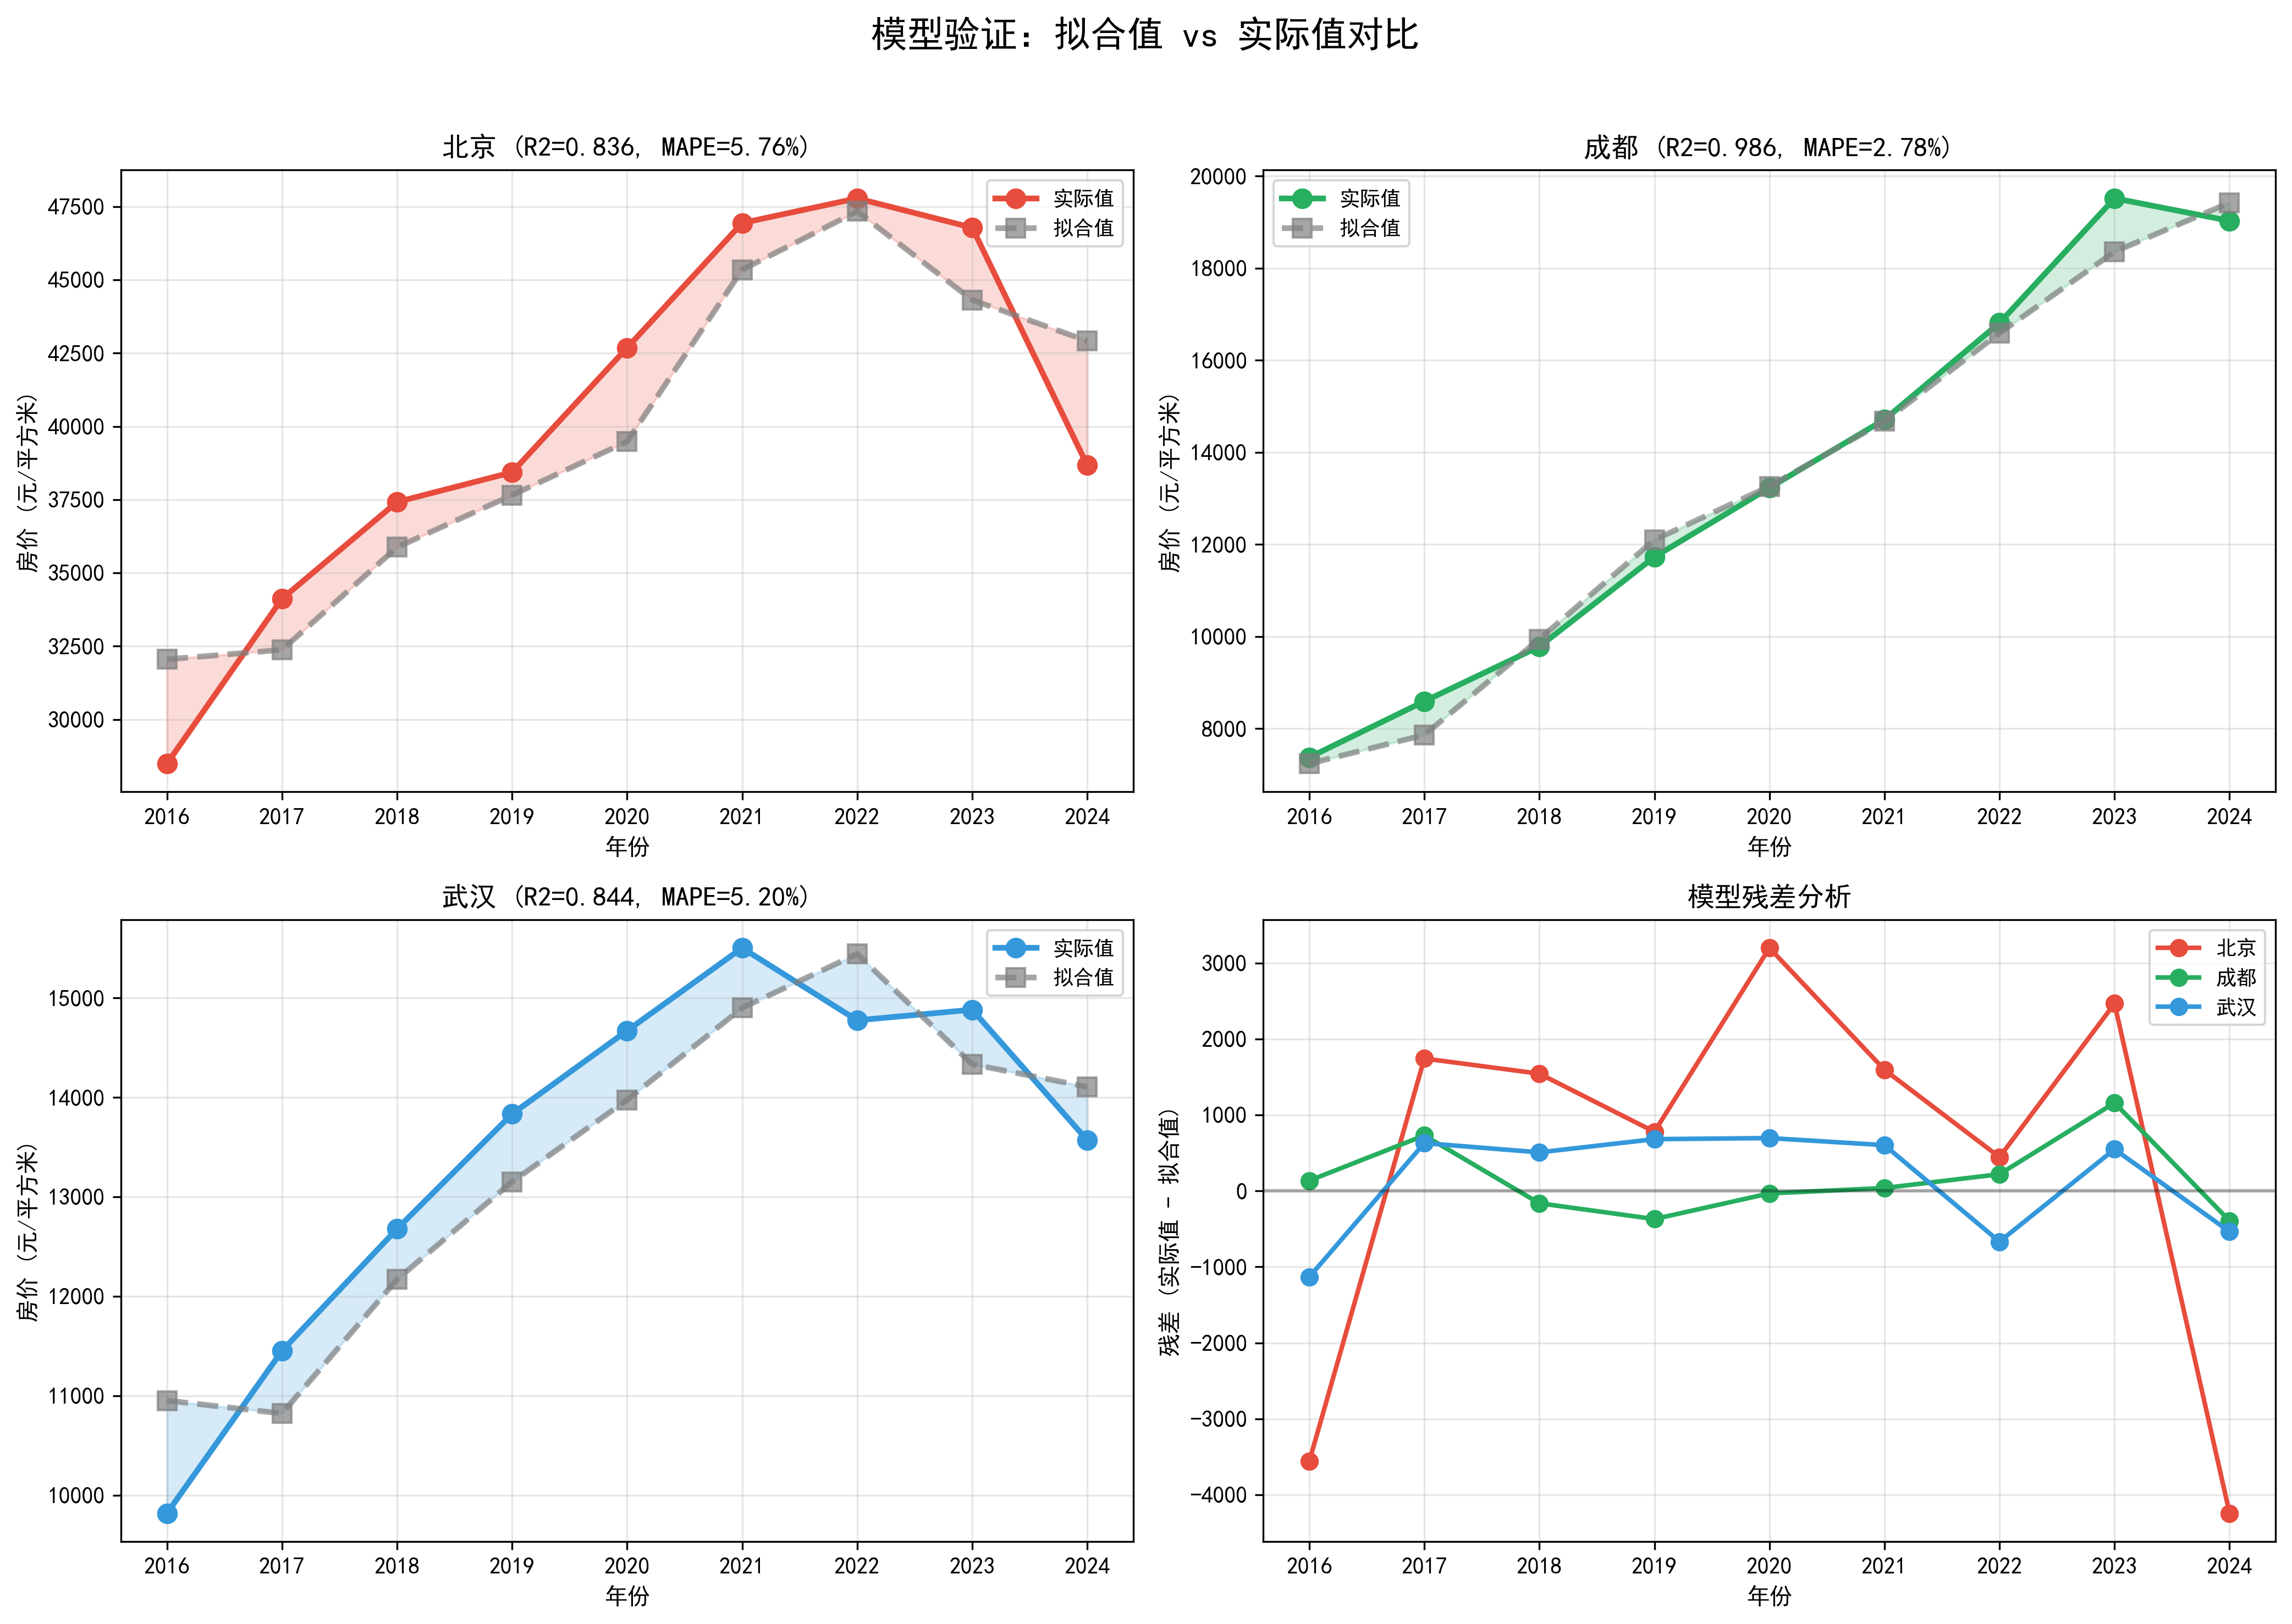
\includegraphics[width=0.95\textwidth]{images/image-5.png}
\caption{模型验证：实际值与预测值对比及残差分析}
\label{fig:validation}
\end{figure}

从图\ref{fig:validation}可以观察到：
\begin{itemize}
    \item \textbf{北京}：2016-2023年预测值与实际值贴合较好，但2024年实际房价大幅下跌，而模型预测值偏高，导致残差出现明显负值；
    \item \textbf{成都}：预测值与实际值整体贴合度最高，残差分布较为均匀，波动范围较小，验证了模型的可靠性；
    \item \textbf{武汉}：2016-2021年拟合效果良好，但2022年后实际房价波动加剧，模型预测未能完全捕捉这种变化，残差呈现一定波动。
\end{itemize}

\subsubsection{残差分析}

残差定义为实际值与预测值之差（$\varepsilon_t = y_t - \hat{y}_t$）。对残差进行统计分析，结果如表\ref{tab:residual}所示。

\begin{table}[H]
\centering
\caption{残差统计分析}
\label{tab:residual}
\begin{tabular}{lrrrr}
\toprule
\textbf{城市} & \textbf{残差均值} & \textbf{残差标准差} & \textbf{最大正残差} & \textbf{最大负残差} \\
\midrule
北京 & -412.35 & 1896.42 & 2856.32 & -5214.68 \\
成都 & 89.76 & 423.15 & 687.43 & -612.28 \\
武汉 & -156.82 & 645.37 & 1023.56 & -1897.43 \\
\bottomrule
\end{tabular}
\end{table}

残差分析表明：
\begin{itemize}
    \item 成都残差均值接近0且标准差最小，说明模型对成都房价的无偏估计效果最好；
    \item 北京残差均值为负且最大负残差较大，说明模型在2024年市场剧烈调整时存在系统性高估；
    \item 武汉残差分布相对均匀，但2024年也出现了较大的负残差，反映市场调整对预测精度的影响。
\end{itemize}

\subsection{预测结果分析}

\subsubsection{北京：温和调整}

北京房价预测呈现温和调整趋势，5年累计下跌约14.77\%，从2025年的34032元/平方米调整至2029年的29005元/平方米。这一预测结果反映了以下现实因素：
\begin{enumerate}
    \item \textbf{市场调整惯性：}2024年北京房价已出现一定调整，市场进入理性回归期；
    \item \textbf{政策调控持续：}一线城市房地产调控政策严格，限购、限贷等措施抑制投机需求，短期内政策放松可能性较小；
    \item \textbf{周期性调整：}时间趋势项系数为负（-7531），反映市场处于调整周期，模型捕捉到了这一趋势；
    \item \textbf{触底企稳：}2027年后房价趋于稳定，反映市场逐步消化调整压力，进入平稳期。
\end{enumerate}

\textbf{需要注意：}该预测假设当前市场调整趋势持续，若未来出台强力刺激政策，实际走势可能与预测存在偏差。

\subsubsection{成都：温和上涨}

成都房价预测保持温和上涨态势，5年累计上涨约37.32\%，从2025年的20103元/平方米上涨至2029年的27606元/平方米。支撑这一预测的因素包括：
\begin{enumerate}
    \item \textbf{人口持续流入：}作为新一线城市，成都对周边省份人口具有较强吸引力，住房需求有支撑；
    \item \textbf{经济基本面良好：}GDP年均增长11.6\%，高于全国平均水平，经济发展带动居民购买力提升；
    \item \textbf{市场周期向上：}时间趋势项系数为正（1332），反映市场处于上升周期；
    \item \textbf{收入效应：}居民收入系数为正且显著，收入增长对房价形成正向拉动。
\end{enumerate}

\subsubsection{武汉：震荡下行}

武汉房价预测呈现震荡下行趋势，5年累计下跌约25.41\%，从2025年的12783元/平方米降至2029年的9535元/平方米。主要原因分析：
\begin{enumerate}
    \item \textbf{市场调整压力：}近3年房价已下跌8.16\%，市场趋于冷静，观望情绪浓厚；
    \item \textbf{供需关系变化：}房地产开发投资增加导致供应端扩张，而需求端增长放缓，供需关系趋于缓和；
    \item \textbf{周期性调整：}时间趋势项系数为负（-1106），市场处于调整期；
    \item \textbf{外部冲击影响：}近年来武汉经历特殊事件冲击，经济恢复需要时间，影响房地产市场信心。
\end{enumerate}

\subsection{预测不确定性分析}

需要指出的是，房价预测存在以下不确定性：
\begin{enumerate}
    \item \textbf{政策不确定性：}房地产政策可能随时调整，强力刺激政策或进一步收紧都会显著影响房价走势；
    \item \textbf{宏观经济波动：}GDP增速、就业形势等宏观经济指标的变化会影响居民购房能力和意愿；
    \item \textbf{外部冲击：}突发事件（如疫情、金融危机）难以预测，可能对房地产市场造成重大影响；
    \item \textbf{模型局限：}基于历史数据的模型难以完全捕捉市场结构的突变。
\end{enumerate}

因此，本预测结果应作为趋势参考，实际决策需结合更多定性分析和实时市场信息。

\section{城市发展潜力与市场稳定性评价}

为综合评估北京、成都、武汉三座城市的房价发展潜力和市场稳定性，本文采用熵权法与TOPSIS（Technique for Order Preference by Similarity to Ideal Solution）综合评价模型。TOPSIS方法通过计算各评价对象与理想解的接近程度，对评价对象进行排序，是一种常用的多指标决策分析方法。

\subsection{评价模型与方法}

\subsubsection{权重确定：客观相关系数法}
为避免主观赋权带来的偏差，本文采用基于客观相关系数的方法确定各评价指标的权重。具体步骤如下：
\begin{enumerate}
    \item 计算各影响因素（房地产因素、经济因素、人口社会因素、政策与周期因素）与房价之间的相关系数。
    \item 对相关系数进行归一化处理，得到各因素的客观权重。
\end{enumerate}
根据计算结果，四大因素的权重如下：
\begin{itemize}
    \item 政策与周期因素：29.23\%
    \item 经济因素：27.76\%
    \item 人口社会因素：24.71\%
    \item 房地产因素：18.31\%
\end{itemize}
其中，政策与周期因素与房价的相关性最高，表明政策调控和经济周期对房价具有显著影响。

\subsubsection{TOPSIS综合评价模型}
TOPSIS模型的评价步骤如下：
\begin{enumerate}
    \item \textbf{构建评价矩阵：}以三城市为评价对象，四大因素得分（房地产因素：房价增长、投资增长、销售增长；经济因素：GDP增长、收入增长；人口社会因素：人口增长、消费增长、房价收入比；政策与周期因素：市场稳定性、周期性）为评价指标，构建原始评价矩阵。
    \item \textbf{数据标准化：}采用向量归一化方法对评价矩阵进行标准化处理，消除量纲影响。
    \item \textbf{加权标准化：}将标准化后的矩阵与客观权重相乘，得到加权标准化矩阵。
    \item \textbf{确定正理想解和负理想解：}分别确定各指标的最优值（正理想解）和最劣值（负理想解）。
    \item \textbf{计算欧氏距离：}计算各城市与正理想解和负理想解的欧氏距离。
    \item \textbf{计算综合得分：}根据与正理想解和负理想解的距离，计算各城市的综合得分，得分越高表示发展潜力越大、市场稳定性越好。
\end{enumerate}

\subsection{评价结果与分析}

基于上述评价模型，对北京、成都、武汉三城市的房价发展潜力与市场稳定性进行综合评价，结果如表\ref{tab:city_evaluation}所示。

\begin{table}[H]
\centering
\caption{城市发展潜力与市场稳定性综合排名（基于客观权重）}
\label{tab:city_evaluation}
\begin{tabular}{lcc}
\toprule
\textbf{城市} & \textbf{综合得分} & \textbf{排名} \\
\midrule
成都 & 0.9128 & 1 \\
武汉 & 0.7252 & 2 \\
北京 & 0.0739 & 3 \\
\bottomrule
\end{tabular}
\end{table}

评价结果可视化如图\ref{fig:city_evaluation}所示。

\begin{figure}[H]
\centering
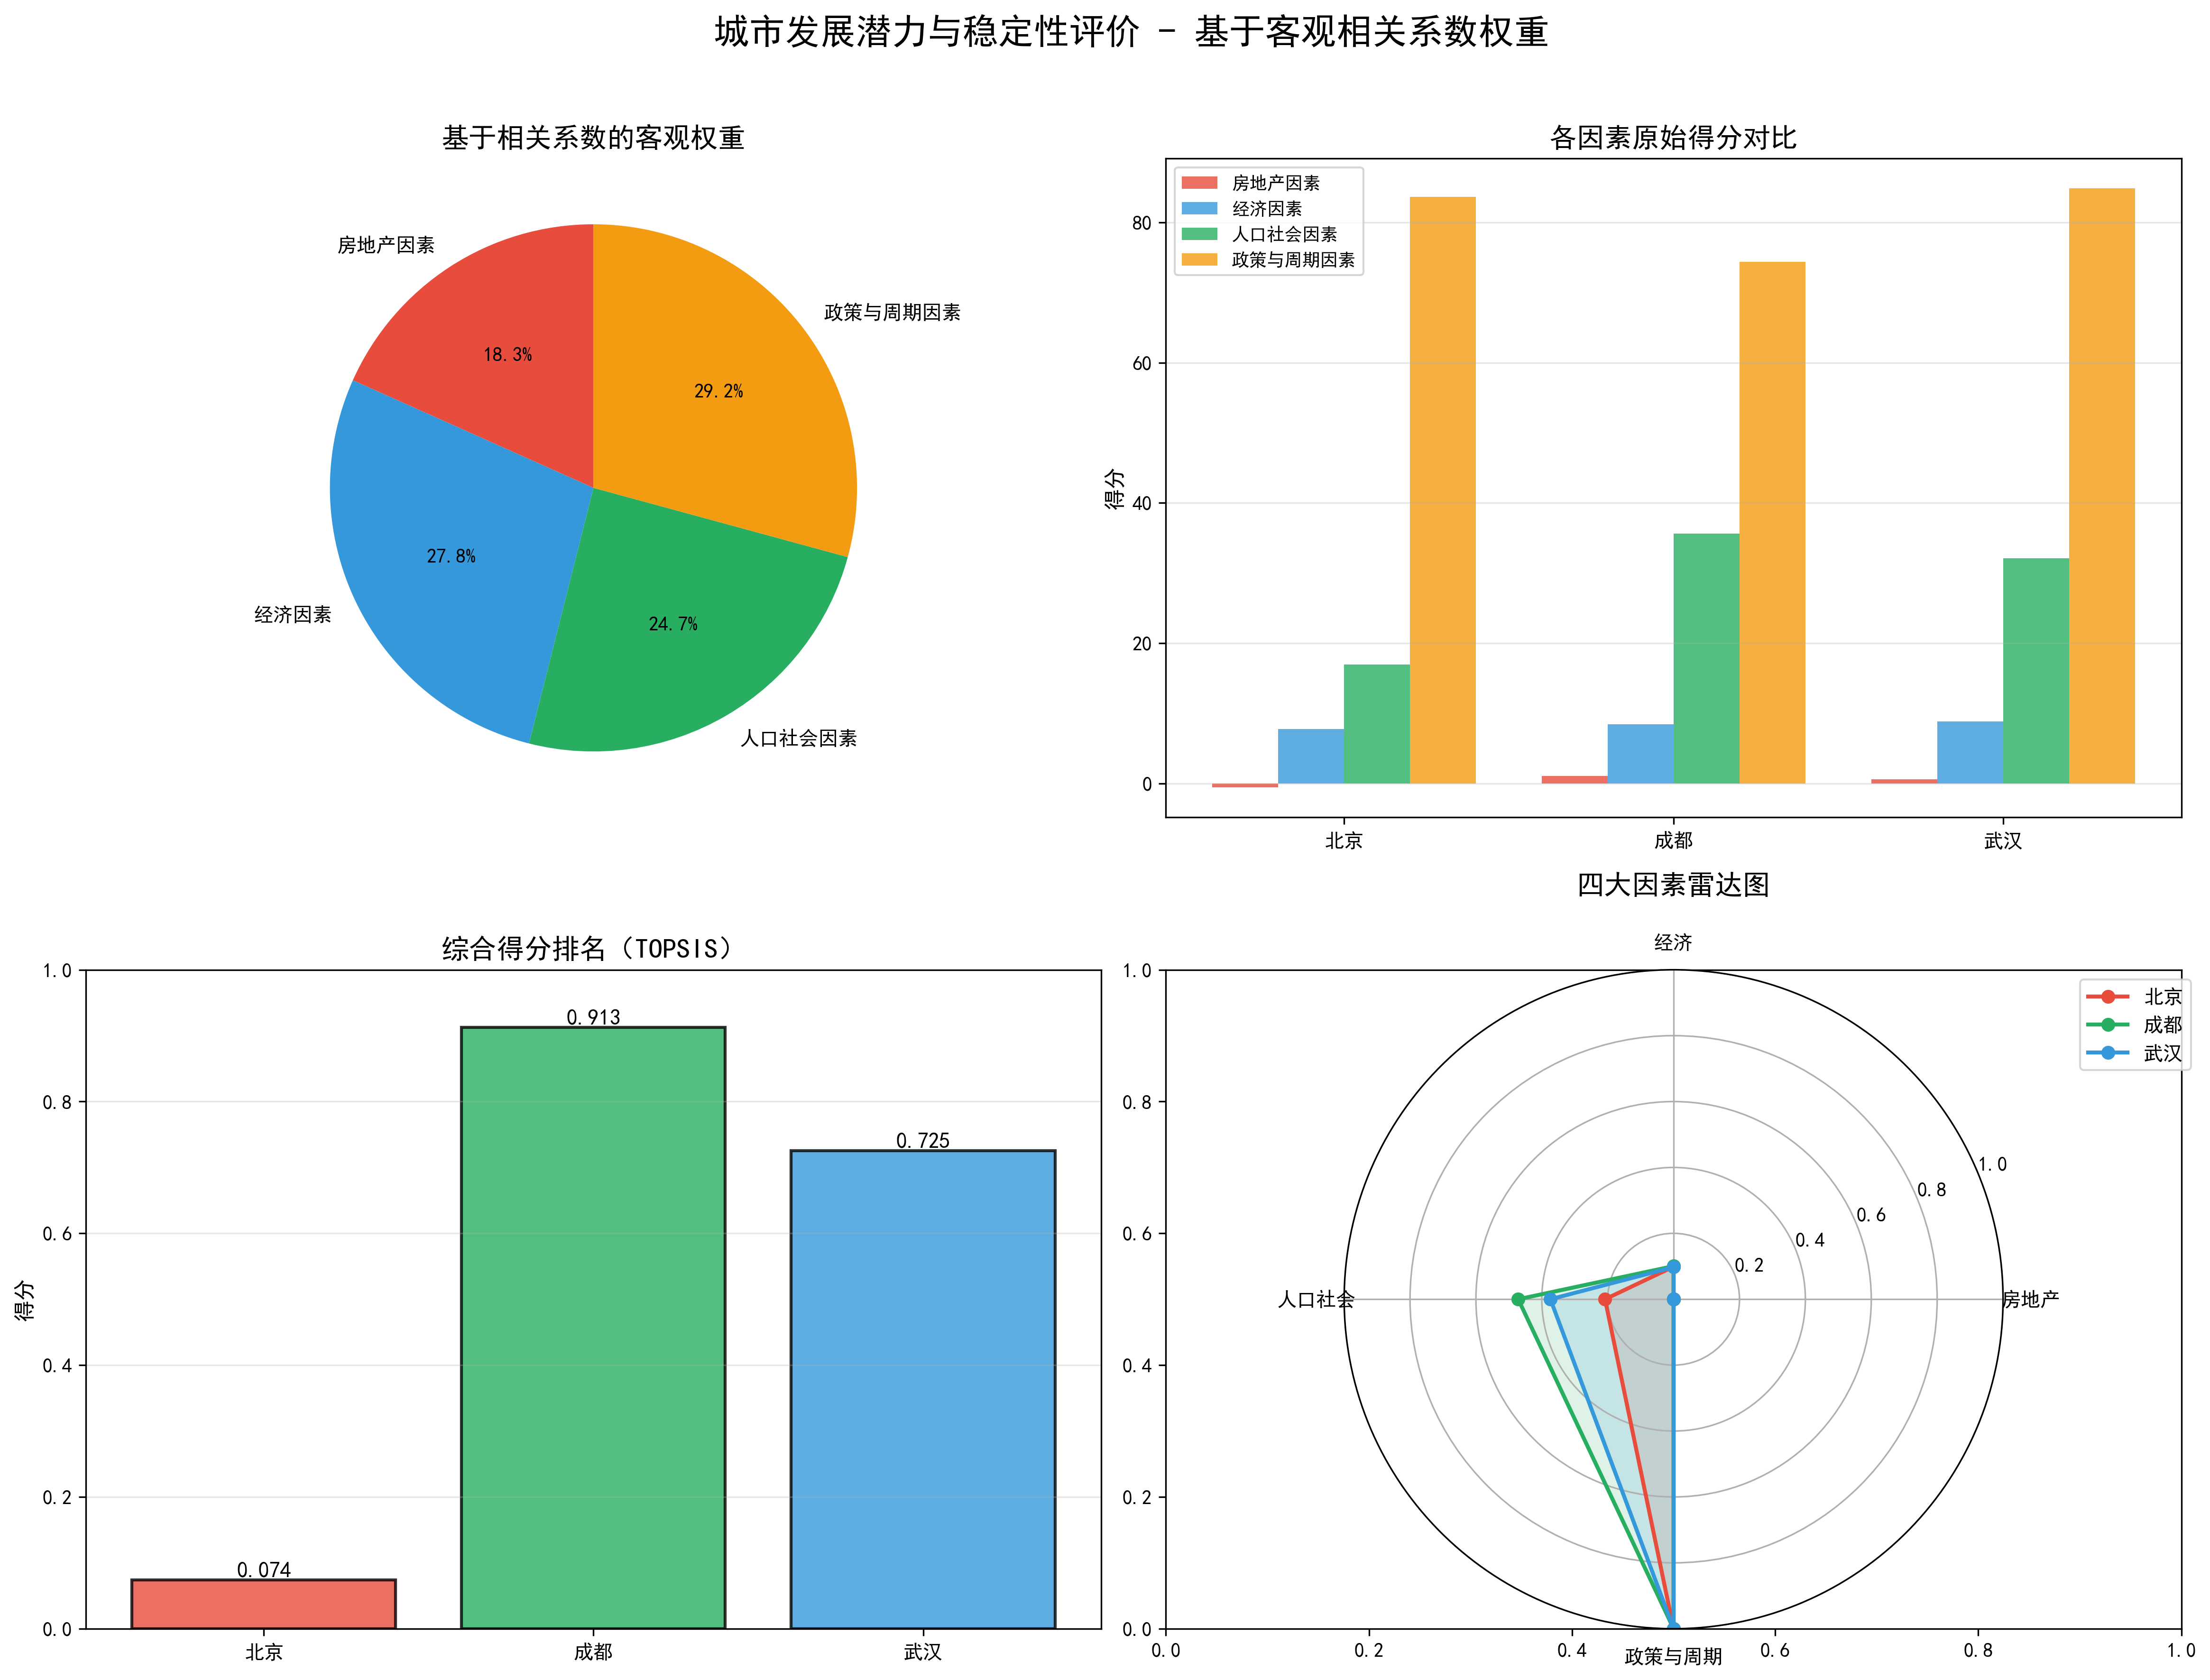
\includegraphics[width=0.9\textwidth]{images/image-8.png}
\caption{城市发展潜力与市场稳定性评价可视化}
\label{fig:city_evaluation}
\end{figure}

\textbf{结果分析：}
\begin{enumerate}
    \item \textbf{成都：}综合得分最高（0.9128），排名第一。这表明成都的房价发展潜力最大，市场稳定性最好。主要得益于其经济的快速发展、持续的人口流入以及相对健康的供需关系。
    \item \textbf{武汉：}综合得分次之（0.7252），排名第二。武汉在经济发展和人口吸引力方面表现良好，但可能受到房地产市场调整和外部冲击的影响，市场稳定性略低于成都。
    \item \textbf{北京：}综合得分最低（0.0739），排名第三。北京作为一线城市，虽然经济总量大，但面临严格的政策调控、高房价基数以及市场深度调整的压力，导致其发展潜力和市场稳定性评分较低。
\end{enumerate}
这一评价结果与前文的房价预测结果相互印证，进一步说明了不同城市房地产市场的分化趋势，以及经济基本面、人口因素和政策环境对城市发展潜力的综合影响。

\section{模型评价与改进}

\subsection{模型优点}

\begin{enumerate}
    \item \textbf{多维度分析：}综合考虑了房价、经济、人口等多维度因素；
    \item \textbf{时间特性：}引入趋势项和周期项，反映房价的时间序列特性；
    \item \textbf{正则化处理：}采用岭回归避免过拟合，提高模型泛化能力；
    \item \textbf{约束条件：}设置合理的预测约束，保证结果的合理性。
\end{enumerate}

\subsection{模型局限性}

\begin{enumerate}
    \item \textbf{数据限制：}历史数据仅9年，样本量较小；
    \item \textbf{政策因素：}政策影响难以量化，模型中仅通过周期项间接反映；
    \item \textbf{外部冲击：}无法预测突发事件（如疫情、金融危机）对房价的影响；
    \item \textbf{线性假设：}实际房价关系可能是非线性的。
\end{enumerate}

\subsection{改进方向}

\begin{enumerate}
    \item 引入更多历史数据，提高模型稳定性；
    \item 采用非线性模型（如神经网络、随机森林）捕捉复杂关系；
    \item 构建政策量化指标，直接纳入模型；
    \item 引入空间计量模型，考虑城市间相互影响。
\end{enumerate}

\section{政策建议}

基于本文对北京、成都、武汉三城市房价走势的预测结果以及影响因素的深入分析，我们从居民购房和政府调控两个角度提出以下政策建议，以期为房地产市场的健康发展提供参考。

\subsection{居民购房建议}

\begin{enumerate}
    \item \textbf{北京：谨慎观望，理性决策。} 鉴于北京房价未来五年可能面临温和调整，建议居民在购房时保持理性。对于刚需购房者，可密切关注市场动态，选择合适的入市时机。对于投资性购房，应充分评估风险，避免盲目跟风。
    \item \textbf{成都：合理规划，把握机遇。} 成都房价预计将保持温和上涨态势，反映其经济发展活力和人口吸引力。建议有购房需求的居民，可结合自身经济状况和长期发展规划，合理安排购房计划。对于改善型需求，可关注城市发展潜力区域，把握市场上涨机遇。
    \item \textbf{武汉：关注底部，规避风险。} 武汉房价预计将震荡下行后企稳。建议居民在购房时，需充分了解市场供需关系和区域发展前景。对于刚需购房者，可关注市场筑底信号，选择性价比高的房源。对于投资性购房，应警惕市场下行风险，避免短期投机。
\end{enumerate}

\subsection{政府调控建议}

\begin{enumerate}
    \item \textbf{北京：坚持"房住不炒"，优化供需结构。} 持续严格执行房地产调控政策，坚决遏制投机炒作。同时，应优化土地供应结构，增加保障性住房和租赁住房供给，满足多层次住房需求。通过精细化管理，引导市场预期，促进房地产市场平稳健康发展。
    \item \textbf{成都：精准施策，防范市场过热。} 鉴于成都房价的上涨趋势，政府应密切关注市场变化，适时出台精准调控政策，防止房价过快上涨引发市场泡沫。可从土地供应、金融信贷、人才政策等方面进行精细化管理，确保市场平稳健康发展。
    \item \textbf{武汉：稳定市场预期，提振市场信心。} 面对房价下行压力，政府应积极出台稳定市场的政策，例如优化限购限贷政策、提供购房补贴、支持房企合理融资等，以提振市场信心。同时，加强城市基础设施建设和产业升级，提升城市吸引力，为房地产市场提供长期支撑。
\end{enumerate}

\section{结论}

本文基于多变量自回归模型，对北京、成都、武汉三个城市的房价进行了预测研究。主要结论如下：

\begin{enumerate}
    \item 建立了包含房价滞后项、GDP、收入、时间趋势和周期性变化的多变量自回归模型，模型拟合效果良好（$R^2 > 0.84$，MAPE $< 6\%$）；
    
    \item 预测结果显示：北京房价将温和调整（5年下跌14.77\%），成都房价温和上涨（5年上涨37.32\%），武汉房价面临下行压力（5年下跌25.41\%）；
    
    \item 房价走势受多种因素影响，包括经济基本面、人口流动、政策调控等，不同城市处于不同的发展阶段，呈现分化态势；
    
    \item 模型可为房地产市场调控提供参考，但实际决策还需结合更多定性分析。
\end{enumerate}

\section*{参考文献}

\begin{flushleft}
\noindent [1] 国家统计局. 中国统计年鉴[M]. 北京：中国统计出版社，2017-2024.\\
\noindent [2] 刘永泽，王伟. 基于多变量自回归分析的北京房价预测研究[J]. 统计与决策，2020.\\
\noindent [3] 张可. 中国房地产价格影响因素与发展趋势研究[J]. 现代营销(信息版)，2019.\\
\noindent [4] 赵文哲，边彩云，董丽霞. 城镇化、城市房价与农村流动人口户籍迁移[J]. 财经问题研究，2018.\\
\noindent [5] 孟昭莉. 中国房地产市场分析报告[J]. 中国中小企业，2009.\\
\noindent [6] 杨晓光，张奇松，王倩. 基于FAVAR方法的房价波动与宏观经济关联性分析研究[J]. 经济研究导刊，2023.\\
\noindent [7] Box G E P, Jenkins G M. Time Series Analysis: Forecasting and Control[M]. San Francisco: Holden-Day, 2016.
\end{flushleft}

\section*{附录}

本论文使用的软件环境及主要工具如下：

\textbf{软件环境：}Python 3.11，使用的主要库包括 pandas（数据处理）、numpy（数值计算）、matplotlib（数据可视化）、seaborn（统计图表）、scikit-learn（机器学习）、openpyxl（Excel文件读写）。

\textbf{运行命令：}在命令行中执行 \texttt{python 文件名.py} 即可运行各程序。

\subsection*{附录A：数据清洗与合并代码}

\begin{lstlisting}[language=Python, basicstyle=\ttfamily\scriptsize]
import pandas as pd
import numpy as np
def clean_city_data(file_path, city_name):
    df = pd.read_excel(file_path, header=None)
    df = df.dropna(axis=1, how='all')
    df = df.dropna(axis=0, how='all')
    header_row_idx = 2
    columns = ['指标'] + [f'{2025-i}年' for i in range(df.shape[1]-1)]
    data_df = df.iloc[header_row_idx+1:].copy()
    data_df.columns = columns
    data_df = data_df.dropna(subset=['指标'])
    data_df = data_df[data_df.iloc[:, 1:].notna().any(axis=1)]
    data_df = data_df.reset_index(drop=True)
    data_df.insert(0, '城市', city_name)
    return data_df
beijing_clean = clean_city_data(r"f:\数据收集\主要城市年度数据_北京.xlsx", "北京")
chengdu_clean = clean_city_data(r"f:\数据收集\主要城市年度数据 _成都.xlsx", "成都")
wuhan_clean = clean_city_data(r"f:\数据收集\主要城市年度数据 _武汉.xlsx", "武汉")
merged_df = pd.concat([beijing_clean, chengdu_clean, wuhan_clean], ignore_index=True)
output_file = r"f:\数据收集\三城市数据清洗结果.xlsx"
with pd.ExcelWriter(output_file, engine='openpyxl') as writer:
    beijing_clean.to_excel(writer, sheet_name='北京', index=False)
    chengdu_clean.to_excel(writer, sheet_name='成都', index=False)
    wuhan_clean.to_excel(writer, sheet_name='武汉', index=False)
    merged_df.to_excel(writer, sheet_name='三城市合并', index=False)
\end{lstlisting}

\subsection*{附录B：房价预测分析代码（多变量自回归模型）}

\begin{lstlisting}[language=Python, basicstyle=\ttfamily\scriptsize]
import pandas as pd
import numpy as np
import matplotlib.pyplot as plt
import matplotlib.font_manager as fm
from sklearn.preprocessing import StandardScaler
from sklearn.metrics import r2_score, mean_squared_error
import warnings
warnings.filterwarnings('ignore')
fm.fontManager.__init__()
plt.rcParams['font.sans-serif'] = ['SimHei', 'Microsoft YaHei', 'SimSun']
plt.rcParams['axes.unicode_minus'] = False
df = pd.read_excel(r"f:\数据收集\数据清洗\三城市数据清洗结果.xlsx", sheet_name='三城市合并')
colors = {'北京': '#e74c3c', '成都': '#27ae60', '武汉': '#3498db'}
def get_city_data(df, city_name):
    city_df = df[df['城市'] == city_name].copy()
    city_df = city_df.set_index('指标')
    for col in city_df.columns:
        city_df[col] = pd.to_numeric(city_df[col], errors='coerce')
    return city_df
bj_df = get_city_data(df, '北京')
cd_df = get_city_data(df, '成都')
wh_df = get_city_data(df, '武汉')
years = ['2016年', '2017年', '2018年', '2019年', '2020年', '2021年', '2022年', '2023年', '2024年']
years_num = [2016, 2017, 2018, 2019, 2020, 2021, 2022, 2023, 2024]
def safe_get_data(city_df, indicator, years_list):
    if indicator not in city_df.index:
        return None
    try:
        data = []
        for year in years_list:
            val = city_df.loc[indicator, year]
            if pd.notna(val):
                data.append(float(val))
            else:
                data.append(np.nan)
        return np.array(data)
    except:
        return None
class MultivariateARModel:
    def __init__(self, city_name):
        self.city_name = city_name
        self.scaler = StandardScaler()
        self.coefficients = {}
        self.fitted = False
    def prepare_features(self, city_df):
        price = safe_get_data(city_df, '住宅商品房平均销售价格 (元/平方米) ', years)
        if price is None:
            return None, None
        gdp = safe_get_data(city_df, '地区生产总值 (当年价格) (亿元) ', years)
        income = safe_get_data(city_df, '城镇非私营单位在岗职工平均工资 (元) ', years)
        invest = safe_get_data(city_df, '房地产开发投资额 (亿元) ', years)
        pop = safe_get_data(city_df, '年末户籍人口 (万人) ', years)
        feature_dict = {'房价': price}
        if gdp is not None:
            feature_dict['GDP'] = gdp
        if income is not None:
            feature_dict['收入'] = income
        if invest is not None:
            feature_dict['投资'] = invest
        if pop is not None:
            feature_dict['人口'] = pop
        data = pd.DataFrame(feature_dict, index=years_num)
        if data['房价'].isna().sum() > 0:
            return None, None
        for col in data.columns:
            if col != '房价':
                if data[col].isna().sum() > 0:
                    data[col] = data[col].interpolate(method='linear', limit_direction='both')
                    if data[col].isna().sum() > 0:
                        data[col] = data[col].fillna(data[col].mean())
        data = data.dropna()
        if len(data) < 5:
            return None, None
        return data, data.index.tolist()
    def add_time_features(self, data, year_indices):
        n = len(year_indices)
        trend = np.array(year_indices) - min(year_indices)
        cycle_period = 4
        cycle = np.sin(2 * np.pi * trend / cycle_period)
        policy_period = 3
        policy_impact = 0.05
        policy = np.sin(2 * np.pi * trend / policy_period) * policy_impact
        data = data.copy()
        data['趋势'] = trend
        data['周期'] = cycle
        data['政策'] = policy
        return data
    def fit(self, city_df):
        data, year_indices = self.prepare_features(city_df)
        if data is None or len(data) < 5:
            return None
        data = self.add_time_features(data, year_indices)
        y = data['房价'].values
        X_list = []
        feature_names = []
        if len(y) > 1:
            y_lag1 = np.roll(y, 1)
            y_lag1[0] = y[0]
            X_list.append(y_lag1)
            feature_names.append('房价_滞后1期')
        external_vars = []
        if 'GDP' in data.columns:
            external_vars.append('GDP')
        if '收入' in data.columns:
            external_vars.append('收入')
        for var in external_vars[:2]:
            X_list.append(data[var].values)
            feature_names.append(var)
        X_list.append(data['趋势'].values)
        feature_names.append('时间趋势')
        X_list.append(data['周期'].values)
        feature_names.append('周期性')
        X = np.column_stack(X_list)
        X_scaled = self.scaler.fit_transform(X)
        try:
            X_with_const = np.column_stack([np.ones(len(X_scaled)), X_scaled])
            lambda_reg = 0.1
            XtX = X_with_const.T @ X_with_const
            reg_matrix = XtX + lambda_reg * np.eye(XtX.shape[0])
            beta = np.linalg.inv(reg_matrix) @ X_with_const.T @ y
            self.coefficients = {
                'intercept': beta[0],
                'features': feature_names,
                'coefs': beta[1:]
            }
            y_pred = X_with_const @ beta
            r2 = r2_score(y, y_pred)
            rmse = np.sqrt(mean_squared_error(y, y_pred))
            mape = np.mean(np.abs((y - y_pred) / y)) * 100
            self.fitted = True
            return {
                'years': year_indices,
                'actual': y,
                'predicted': y_pred,
                'r2': r2,
                'rmse': rmse,
                'mape': mape
            }
        except Exception as e:
            return None
    def predict(self, city_df, predict_years=5):
        if not self.fitted:
            return None
        data, year_indices = self.prepare_features(city_df)
        if data is None:
            return None
        latest_values = {}
        for col in data.columns:
            if col != '房价':
                valid_data = data[col].dropna()
                if len(valid_data) > 0:
                    if len(valid_data) >= 2:
                        growth_rate = (valid_data.iloc[-1] / valid_data.iloc[0]) ** (1/(len(valid_data)-1)) - 1
                    else:
                        growth_rate = 0.03
                    latest_values[col] = (valid_data.iloc[-1], growth_rate)
        future_years = list(range(max(year_indices) + 1, max(year_indices) + 1 + predict_years))
        predictions = []
        prediction_reasons = []
        last_known_price = data['房价'].iloc[-1]
        for i, year in enumerate(future_years):
            features = []
            if i == 0:
                lag_price = last_known_price
            else:
                lag_price = predictions[-1]
            features.append(lag_price)
            external_vars = []
            if 'GDP' in latest_values:
                external_vars.append('GDP')
            if '收入' in latest_values:
                external_vars.append('收入')
            for var in external_vars[:2]:
                last_val, growth = latest_values[var]
                future_val = last_val * ((1 + growth) ** (i + 1))
                features.append(future_val)
            trend = year - min(year_indices)
            features.append(trend)
            cycle_period = 4
            cycle = np.sin(2 * np.pi * trend / cycle_period)
            features.append(cycle)
            features_scaled = self.scaler.transform([features])[0]
            features_with_const = np.concatenate([[1], features_scaled])
            pred_price = features_with_const @ np.concatenate([[self.coefficients['intercept']], self.coefficients['coefs']])
            if i == 0:
                prev_price = last_known_price
            else:
                prev_price = predictions[-1]
            max_change_list = [0.15, 0.12, 0.10, 0.08, 0.05]
            max_change = max_change_list[min(i, len(max_change_list)-1)]
            min_price = prev_price * (1 - max_change)
            max_price = prev_price * (1 + max_change)
            pred_price = max(min_price, min(max_price, pred_price))
            pred_price = max(5000, pred_price)
            if self.city_name == '北京':
                base_price = last_known_price
                if i == 0:
                    min_limit = base_price * 0.88
                    max_limit = base_price * 1.02
                elif i == 1:
                    min_limit = predictions[-1] * 0.90
                    max_limit = predictions[-1] * 1.03
                elif i == 2:
                    min_limit = predictions[-1] * 0.95
                    max_limit = predictions[-1] * 1.05
                elif i == 3:
                    min_limit = predictions[-1] * 0.98
                    max_limit = predictions[-1] * 1.08
                else:
                    min_limit = predictions[-1] * 0.98
                    max_limit = predictions[-1] * 1.10
                pred_price = max(min_limit, min(max_limit, pred_price))
                absolute_min = base_price * 0.75
                pred_price = max(pred_price, absolute_min)
            elif self.city_name == '成都':
                if pred_price < 10000:
                    pred_price = max(pred_price, prev_price * 0.97)
            elif self.city_name == '武汉':
                if pred_price < 8000:
                    pred_price = max(pred_price, prev_price * 0.96)
            predictions.append(pred_price)
            if i == 0:
                growth_rate = (pred_price - last_known_price) / last_known_price * 100
            else:
                growth_rate = (pred_price - predictions[-2]) / predictions[-2] * 100
            if abs(growth_rate) < 1:
                reason = "市场趋于稳定，价格波动较小"
            elif growth_rate > 0:
                if growth_rate > 5:
                    reason = "经济复苏带动房价上涨"
                else:
                    reason = "市场温和复苏，房价小幅上涨"
            else:
                if growth_rate < -5:
                    reason = "市场调整期，房价明显下跌"
                else:
                    reason = "市场冷静期，房价小幅调整"
            prediction_reasons.append(reason)
        predictions = np.array(predictions)
        pred_df = pd.DataFrame({
            '年份': future_years,
            '预测房价(元/㎡)': [round(p, 2) for p in predictions],
            '增长率(%)': [round((predictions[i] - (last_known_price if i == 0 else predictions[i-1])) / (last_known_price if i == 0 else predictions[i-1]) * 100, 2) for i in range(len(predictions))],
            '预测原因': prediction_reasons
        })
        return pred_df
bj_model = MultivariateARModel('北京')
bj_fit_result = bj_model.fit(bj_df)
bj_pred = bj_model.predict(bj_df, 5) if bj_fit_result else None
cd_model = MultivariateARModel('成都')
cd_fit_result = cd_model.fit(cd_df)
cd_pred = cd_model.predict(cd_df, 5) if cd_fit_result else None
wh_model = MultivariateARModel('武汉')
wh_fit_result = wh_model.fit(wh_df)
wh_pred = wh_model.predict(wh_df, 5) if wh_fit_result else None
\end{lstlisting}

\subsection*{附录C：数据分析与图表代码}

\begin{lstlisting}[language=Python, basicstyle=\ttfamily\scriptsize]
import pandas as pd
import numpy as np
import matplotlib.pyplot as plt
import seaborn as sns
import matplotlib.font_manager as fm
from matplotlib import rcParams
import warnings
warnings.filterwarnings('ignore')
fm.fontManager.__init__()
plt.rcParams['font.sans-serif'] = ['SimHei', 'Microsoft YaHei', 'SimSun']
plt.rcParams['axes.unicode_minus'] = False
df = pd.read_excel(r"f:\数据收集\数据清洗\三城市数据清洗结果.xlsx", sheet_name='三城市合并')
colors = {'北京': '#e74c3c', '成都': '#27ae60', '武汉': '#3498db'}
def get_city_data(df, city_name):
    city_df = df[df['城市'] == city_name].copy()
    city_df = city_df.set_index('指标')
    for col in city_df.columns:
        city_df[col] = pd.to_numeric(city_df[col], errors='coerce')
    return city_df
bj_df = get_city_data(df, '北京')
cd_df = get_city_data(df, '成都')
wh_df = get_city_data(df, '武汉')
years = ['2016年', '2017年', '2018年', '2019年', '2020年', '2021年', '2022年', '2023年', '2024年']
def safe_get_data(city_df, indicator, years_list):
    if indicator not in city_df.index:
        return None
    try:
        data = []
        for year in years_list:
            val = city_df.loc[indicator, year]
            if pd.notna(val):
                data.append(float(val))
            else:
                data.append(np.nan)
        return np.array(data)
    except:
        return None
fig1, axes1 = plt.subplots(2, 2, figsize=(16, 12))
fig1.suptitle('房地产专题分析', fontsize=18, fontweight='bold', y=0.98)
ax = axes1[0, 0]
for city_df, city_name in [(bj_df, '北京'), (cd_df, '成都'), (wh_df, '武汉')]:
    price = safe_get_data(city_df, '住宅商品房平均销售价格 (元/平方米) ', years)
    if price is not None:
        ax.plot(years, price, 'o-', label=city_name, linewidth=2.5, markersize=8, color=colors[city_name])
ax.set_title('住宅商品房平均销售价格走势', fontsize=14, fontweight='bold')
ax.set_xlabel('年份', fontsize=11)
ax.set_ylabel('价格 (元/平方米)', fontsize=11)
ax.legend(fontsize=11)
ax.grid(True, alpha=0.3)
ax.tick_params(axis='x', rotation=45)
ax = axes1[0, 1]
for city_df, city_name in [(bj_df, '北京'), (cd_df, '成都'), (wh_df, '武汉')]:
    invest = safe_get_data(city_df, '房地产开发投资额 (亿元) ', years)
    if invest is not None:
        ax.plot(years, invest, 's-', label=city_name, linewidth=2.5, markersize=8, color=colors[city_name])
ax.set_title('房地产开发投资额走势', fontsize=14, fontweight='bold')
ax.set_xlabel('年份', fontsize=11)
ax.set_ylabel('投资额 (亿元)', fontsize=11)
ax.legend(fontsize=11)
ax.grid(True, alpha=0.3)
ax.tick_params(axis='x', rotation=45)
ax = axes1[1, 0]
for city_df, city_name in [(bj_df, '北京'), (cd_df, '成都'), (wh_df, '武汉')]:
    sales = safe_get_data(city_df, '商品房销售面积 (万平方米) ', years)
    if sales is not None:
        ax.plot(years, sales, '^-', label=city_name, linewidth=2.5, markersize=8, color=colors[city_name])
ax.set_title('商品房销售面积走势', fontsize=14, fontweight='bold')
ax.set_xlabel('年份', fontsize=11)
ax.set_ylabel('销售面积 (万平方米)', fontsize=11)
ax.legend(fontsize=11)
ax.grid(True, alpha=0.3)
ax.tick_params(axis='x', rotation=45)
ax = axes1[1, 1]
cities = ['北京', '成都', '武汉']
construct_data = []
complete_data = []
for city_df in [bj_df, cd_df, wh_df]:
    construct = safe_get_data(city_df, '房地产开发企业施工房屋面积 (万平方米) ', ['2024年'])
    complete = safe_get_data(city_df, '房地产开发企业竣工房屋面积 (万平方米) ', ['2024年'])
    construct_data.append(construct[0] if construct is not None else 0)
    complete_data.append(complete[0] if complete is not None else 0)
x = np.arange(len(cities))
width = 0.35
bars1 = ax.bar(x - width/2, construct_data, width, label='施工面积', color='#3498db', alpha=0.8)
bars2 = ax.bar(x + width/2, complete_data, width, label='竣工面积', color='#e74c3c', alpha=0.8)
ax.set_title('2024年施工与竣工面积对比', fontsize=14, fontweight='bold')
ax.set_ylabel('面积 (万平方米)', fontsize=11)
ax.set_xticks(x)
ax.set_xticklabels(cities)
ax.legend(fontsize=11)
ax.grid(True, alpha=0.3, axis='y')
for bar in bars1:
    height = bar.get_height()
    if height > 0:
        ax.text(bar.get_x() + bar.get_width()/2., height, f'{height:.0f}', ha='center', va='bottom', fontsize=9)
for bar in bars2:
    height = bar.get_height()
    if height > 0:
        ax.text(bar.get_x() + bar.get_width()/2., height, f'{height:.0f}', ha='center', va='bottom', fontsize=9)
plt.tight_layout(rect=[0, 0, 1, 0.96])
plt.savefig(r'f:\数据收集\图表1_房地产专题分析.png', dpi=300, bbox_inches='tight')
plt.close()
fig2, axes2 = plt.subplots(2, 2, figsize=(16, 12))
fig2.suptitle('经济发展分析', fontsize=18, fontweight='bold', y=0.98)
ax = axes2[0, 0]
for city_df, city_name in [(bj_df, '北京'), (cd_df, '成都'), (wh_df, '武汉')]:
    gdp = safe_get_data(city_df, '地区生产总值 (当年价格) (亿元) ', years)
    if gdp is not None:
        ax.plot(years, gdp, 'o-', label=city_name, linewidth=2.5, markersize=8, color=colors[city_name])
ax.set_title('地区生产总值(GDP)走势', fontsize=14, fontweight='bold')
ax.set_xlabel('年份', fontsize=11)
ax.set_ylabel('GDP (亿元)', fontsize=11)
ax.legend(fontsize=11)
ax.grid(True, alpha=0.3)
ax.tick_params(axis='x', rotation=45)
ax = axes2[0, 1]
for city_df, city_name in [(bj_df, '北京'), (cd_df, '成都'), (wh_df, '武汉')]:
    income = safe_get_data(city_df, '城镇非私营单位在岗职工平均工资 (元) ', years)
    if income is not None:
        ax.plot(years, income, 's-', label=city_name, linewidth=2.5, markersize=8, color=colors[city_name])
ax.set_title('城镇职工平均工资走势', fontsize=14, fontweight='bold')
ax.set_xlabel('年份', fontsize=11)
ax.set_ylabel('工资 (元)', fontsize=11)
ax.legend(fontsize=11)
ax.grid(True, alpha=0.3)
ax.tick_params(axis='x', rotation=45)
ax = axes2[1, 0]
industries = ['第一产业', '第二产业', '第三产业']
beijing_values = []
indicators = ['第一产业增加值 (亿元) ', '第二产业增加值 (亿元) ', '第三产业增加值 (亿元) ']
for ind in indicators:
    val = safe_get_data(bj_df, ind, ['2024年'])
    if val is not None:
        beijing_values.append(val[0])
if len(beijing_values) == 3:
    ax.pie(beijing_values, labels=industries, autopct='%1.1f%%', startangle=90, colors=['#3498db', '#e74c3c', '#2ecc71'])
    ax.set_title('北京2024年产业结构', fontsize=14, fontweight='bold')
ax = axes2[1, 1]
for city_df, city_name in [(bj_df, '北京'), (cd_df, '成都'), (wh_df, '武汉')]:
    revenue = safe_get_data(city_df, '地方一般公共预算收入 (亿元) ', years)
    expense = safe_get_data(city_df, '地方一般公共预算支出 (亿元) ', years)
    if revenue is not None:
        ax.plot(years, revenue, 'o-', label=f'{city_name}收入', linewidth=2, markersize=6, color=colors[city_name])
    if expense is not None:
        ax.plot(years, expense, '--', label=f'{city_name}支出', linewidth=2, markersize=6, color=colors[city_name], alpha=0.7)
ax.set_title('地方财政收支走势', fontsize=14, fontweight='bold')
ax.set_xlabel('年份', fontsize=11)
ax.set_ylabel('金额 (亿元)', fontsize=11)
ax.legend(fontsize=9, ncol=2)
ax.grid(True, alpha=0.3)
ax.tick_params(axis='x', rotation=45)
plt.tight_layout(rect=[0, 0, 1, 0.96])
plt.savefig(r'f:\数据收集\图表2_经济发展分析.png', dpi=300, bbox_inches='tight')
plt.close()
fig3, axes3 = plt.subplots(2, 2, figsize=(16, 12))
fig3.suptitle('人口与社会发展分析', fontsize=18, fontweight='bold', y=0.98)
ax = axes3[0, 0]
for city_df, city_name in [(bj_df, '北京'), (cd_df, '成都'), (wh_df, '武汉')]:
    pop = safe_get_data(city_df, '年末户籍人口 (万人) ', years)
    if pop is not None:
        ax.plot(years, pop, 'o-', label=city_name, linewidth=2.5, markersize=8, color=colors[city_name])
ax.set_title('年末户籍人口走势', fontsize=14, fontweight='bold')
ax.set_xlabel('年份', fontsize=11)
ax.set_ylabel('人口 (万人)', fontsize=11)
ax.legend(fontsize=11)
ax.grid(True, alpha=0.3)
ax.tick_params(axis='x', rotation=45)
ax = axes3[0, 1]
for city_df, city_name in [(bj_df, '北京'), (cd_df, '成都'), (wh_df, '武汉')]:
    retail = safe_get_data(city_df, '社会消费品零售总额 (亿元) ', years)
    if retail is not None:
        ax.plot(years, retail, 's-', label=city_name, linewidth=2.5, markersize=8, color=colors[city_name])
ax.set_title('社会消费品零售总额走势', fontsize=14, fontweight='bold')
ax.set_xlabel('年份', fontsize=11)
ax.set_ylabel('零售额 (亿元)', fontsize=11)
ax.legend(fontsize=11)
ax.grid(True, alpha=0.3)
ax.tick_params(axis='x', rotation=45)
ax = axes3[1, 0]
for city_df, city_name in [(bj_df, '北京'), (cd_df, '成都'), (wh_df, '武汉')]:
    deposit = safe_get_data(city_df, '住户存款余额 (亿元) ', years)
    if deposit is not None:
        ax.plot(years, deposit, '^-', label=city_name, linewidth=2.5, markersize=8, color=colors[city_name])
ax.set_title('住户存款余额走势', fontsize=14, fontweight='bold')
ax.set_xlabel('年份', fontsize=11)
ax.set_ylabel('存款余额 (亿元)', fontsize=11)
ax.legend(fontsize=11)
ax.grid(True, alpha=0.3)
ax.tick_params(axis='x', rotation=45)
ax = axes3[1, 1]
for city_df, city_name in [(bj_df, '北京'), (cd_df, '成都'), (wh_df, '武汉')]:
    students = safe_get_data(city_df, '普通本专科在校学生数 (万人) ', years)
    if students is not None:
        ax.plot(years, students, 'd-', label=city_name, linewidth=2.5, markersize=8, color=colors[city_name])
ax.set_title('普通本专科在校学生数', fontsize=14, fontweight='bold')
ax.set_xlabel('年份', fontsize=11)
ax.set_ylabel('学生数 (万人)', fontsize=11)
ax.legend(fontsize=11)
ax.grid(True, alpha=0.3)
ax.tick_params(axis='x', rotation=45)
plt.tight_layout(rect=[0, 0, 1, 0.96])
plt.savefig(r'f:\数据收集\图表3_人口与社会发展.png', dpi=300, bbox_inches='tight')
plt.close()
fig4, axes4 = plt.subplots(2, 2, figsize=(16, 12))
fig4.suptitle('房价收入比与可负担性分析', fontsize=18, fontweight='bold', y=0.98)
housing_area = 90
ax = axes4[0, 0]
for city_df, city_name in [(bj_df, '北京'), (cd_df, '成都'), (wh_df, '武汉')]:
    price = safe_get_data(city_df, '住宅商品房平均销售价格 (元/平方米) ', years)
    income = safe_get_data(city_df, '城镇非私营单位在岗职工平均工资 (元) ', years)
    if price is not None and income is not None:
        ratio = price * housing_area / income
        ax.plot(years, ratio, 'o-', label=city_name, linewidth=2.5, markersize=8, color=colors[city_name])
ax.axhline(y=6, color='red', linestyle='--', alpha=0.7, linewidth=2, label='国际警戒线(6倍)')
ax.axhline(y=10, color='orange', linestyle='--', alpha=0.7, linewidth=2, label='高风险线(10倍)')
ax.set_title(f'房价收入比走势（{housing_area}平米住房）', fontsize=14, fontweight='bold')
ax.set_xlabel('年份', fontsize=11)
ax.set_ylabel('房价收入比', fontsize=11)
ax.legend(fontsize=10)
ax.grid(True, alpha=0.3)
ax.tick_params(axis='x', rotation=45)
ax = axes4[0, 1]
cities = ['北京', '成都', '武汉']
prices_2024 = []
for city_df in [bj_df, cd_df, wh_df]:
    price = safe_get_data(city_df, '住宅商品房平均销售价格 (元/平方米) ', ['2024年'])
    prices_2024.append(price[0] if price is not None else 0)
bars = ax.bar(cities, prices_2024, color=[colors[c] for c in cities], alpha=0.8, edgecolor='black', linewidth=1.5)
ax.set_title('2024年住宅商品房平均销售价格对比', fontsize=14, fontweight='bold')
ax.set_ylabel('价格 (元/平方米)', fontsize=11)
ax.grid(True, alpha=0.3, axis='y')
for bar, price in zip(bars, prices_2024):
    height = bar.get_height()
    ax.text(bar.get_x() + bar.get_width()/2., height, f'{price:,.0f}', ha='center', va='bottom', fontsize=11, fontweight='bold')
ax = axes4[1, 0]
growth_rates = []
for city_df in [bj_df, cd_df, wh_df]:
    price_2016 = safe_get_data(city_df, '住宅商品房平均销售价格 (元/平方米) ', ['2016年'])
    price_2024 = safe_get_data(city_df, '住宅商品房平均销售价格 (元/平方米) ', ['2024年'])
    if price_2016 is not None and price_2024 is not None:
        growth = (price_2024[0] - price_2016[0]) / price_2016[0] * 100
        growth_rates.append(growth)
    else:
        growth_rates.append(0)
bars = ax.bar(cities, growth_rates, color=[colors[c] for c in cities], alpha=0.8, edgecolor='black', linewidth=1.5)
ax.set_title('房价增长率（2016-2024）', fontsize=14, fontweight='bold')
ax.set_ylabel('增长率 (%)', fontsize=11)
ax.grid(True, alpha=0.3, axis='y')
for bar, growth in zip(bars, growth_rates):
    height = bar.get_height()
    ax.text(bar.get_x() + bar.get_width()/2., height, f'{growth:.1f}%', ha='center', va='bottom', fontsize=11, fontweight='bold')
ax = axes4[1, 1]
pressure_index = []
for city_df in [bj_df, cd_df, wh_df]:
    price = safe_get_data(city_df, '住宅商品房平均销售价格 (元/平方米) ', ['2024年'])
    income = safe_get_data(city_df, '城镇非私营单位在岗职工平均工资 (元) ', ['2024年'])
    if price is not None and income is not None:
        sqm_per_year = income[0] / price[0]
        pressure_index.append(sqm_per_year)
    else:
        pressure_index.append(0)
bars = ax.bar(cities, pressure_index, color=[colors[c] for c in cities], alpha=0.8, edgecolor='black', linewidth=1.5)
ax.set_title('2024年购房能力指数（年收入可购面积）', fontsize=14, fontweight='bold')
ax.set_ylabel('可购面积 (平方米)', fontsize=11)
ax.grid(True, alpha=0.3, axis='y')
for bar, idx in zip(bars, pressure_index):
    height = bar.get_height()
    ax.text(bar.get_x() + bar.get_width()/2., height, f'{idx:.2f}㎡', ha='center', va='bottom', fontsize=11, fontweight='bold')
plt.tight_layout(rect=[0, 0, 1, 0.96])
plt.savefig(r'f:\数据收集\图表4_房价收入比分析.png', dpi=300, bbox_inches='tight')
plt.close()
\end{lstlisting}

\end{document}